%%%%%%%%%%%%%%%%%%%%%%%%%%%
% Do Elections Affect Fed Forecasts?
% Cassandra Grafström and Christopher Gandrud
%%%%%%%%%%%%%%%%%%%%%%%%%%%%

% !Rnw weave = knitr

\documentclass[a4paper]{article}\usepackage{graphicx, color}
%% maxwidth is the original width if it is less than linewidth
%% otherwise use linewidth (to make sure the graphics do not exceed the margin)
\makeatletter
\def\maxwidth{ %
  \ifdim\Gin@nat@width>\linewidth
    \linewidth
  \else
    \Gin@nat@width
  \fi
}
\makeatother

\IfFileExists{upquote.sty}{\usepackage{upquote}}{}
\definecolor{fgcolor}{rgb}{0.2, 0.2, 0.2}
\newcommand{\hlnumber}[1]{\textcolor[rgb]{0,0,0}{#1}}%
\newcommand{\hlfunctioncall}[1]{\textcolor[rgb]{0.501960784313725,0,0.329411764705882}{\textbf{#1}}}%
\newcommand{\hlstring}[1]{\textcolor[rgb]{0.6,0.6,1}{#1}}%
\newcommand{\hlkeyword}[1]{\textcolor[rgb]{0,0,0}{\textbf{#1}}}%
\newcommand{\hlargument}[1]{\textcolor[rgb]{0.690196078431373,0.250980392156863,0.0196078431372549}{#1}}%
\newcommand{\hlcomment}[1]{\textcolor[rgb]{0.180392156862745,0.6,0.341176470588235}{#1}}%
\newcommand{\hlroxygencomment}[1]{\textcolor[rgb]{0.43921568627451,0.47843137254902,0.701960784313725}{#1}}%
\newcommand{\hlformalargs}[1]{\textcolor[rgb]{0.690196078431373,0.250980392156863,0.0196078431372549}{#1}}%
\newcommand{\hleqformalargs}[1]{\textcolor[rgb]{0.690196078431373,0.250980392156863,0.0196078431372549}{#1}}%
\newcommand{\hlassignement}[1]{\textcolor[rgb]{0,0,0}{\textbf{#1}}}%
\newcommand{\hlpackage}[1]{\textcolor[rgb]{0.588235294117647,0.709803921568627,0.145098039215686}{#1}}%
\newcommand{\hlslot}[1]{\textit{#1}}%
\newcommand{\hlsymbol}[1]{\textcolor[rgb]{0,0,0}{#1}}%
\newcommand{\hlprompt}[1]{\textcolor[rgb]{0.2,0.2,0.2}{#1}}%

\usepackage{framed}
\makeatletter
\newenvironment{kframe}{%
 \def\at@end@of@kframe{}%
 \ifinner\ifhmode%
  \def\at@end@of@kframe{\end{minipage}}%
  \begin{minipage}{\columnwidth}%
 \fi\fi%
 \def\FrameCommand##1{\hskip\@totalleftmargin \hskip-\fboxsep
 \colorbox{shadecolor}{##1}\hskip-\fboxsep
     % There is no \\@totalrightmargin, so:
     \hskip-\linewidth \hskip-\@totalleftmargin \hskip\columnwidth}%
 \MakeFramed {\advance\hsize-\width
   \@totalleftmargin\z@ \linewidth\hsize
   \@setminipage}}%
 {\par\unskip\endMakeFramed%
 \at@end@of@kframe}
\makeatother

\definecolor{shadecolor}{rgb}{.97, .97, .97}
\definecolor{messagecolor}{rgb}{0, 0, 0}
\definecolor{warningcolor}{rgb}{1, 0, 1}
\definecolor{errorcolor}{rgb}{1, 0, 0}
\newenvironment{knitrout}{}{} % an empty environment to be redefined in TeX

\usepackage{alltt}
\usepackage{fullpage}
\usepackage[authoryear]{natbib}
\usepackage{setspace}
    \doublespacing
\usepackage[usenames,dvipsnames]{xcolor}
\usepackage{hyperref}
\hypersetup{
    colorlinks,
    citecolor=black,
    filecolor=black,
    linkcolor=cyan,
    urlcolor=cyan
}
\usepackage{dcolumn}
\usepackage{booktabs}
\usepackage{url}
\usepackage{tikz}
\usepackage{todonotes}
\usepackage[utf8]{inputenc} 

%%%%%%% Title Page %%%%%%%%%%%%%%%%%%%%%%%%%%%%%%%%%%%%%%%%%%%%
\title{Does Presidential Partisanship Affect Fed Inflation Forecasts?}

\author{Christopher Gandrud \\
                {\emph{Yonsei University}}\footnote{\href{mailto:gandrud@yonsei.ac.kr}{gandrud@yonsei.ac.kr}} \\
                and \\
            Cassandra Grafstr\"{o}m \\
                {\emph{Hertie School of Governance \& University of Michigan}}\footnote{\href{mailto:cgrafstr@umich.edu}{cgrafstr@umich.edu}}}

\begin{document}



\maketitle

%%%%%%% Abstract %%%%%%%%%%%%%%%%%%%%%%%%%%%%%%%%%%%%%%%%%%%%
\begin{abstract}
\noindent\emph{Working paper prepared for the APSA Annual Conference 2012. \\ Comments welcome.}\footnote{Thank you to the Mark Hallerberg and the Fiscal Governance Centre at the Hertie School of Governance for support. Thank you also to Thomas Stark and seminar participants at the London School of Economics and Yonsei University.} \\[0.2cm]

Recent work argues that policy-makers at the United States Federal Reserve are not politically indifferent \citep{Clark2012}. The Fed tends to choose looser monetary policies during Republican administrations, possibly in order to ensure the (re)election of ideologically preferred presidents. This model excludes an essential aspect of monetary policy decision-making: expectations about future inflation. We use the Fed's Green Book forecasts to test whether presidents' partisan identification shapes the estimates of future economic performance that influence FOMC policies. We find that Federal Reserve staff probably {\emph{do not}} bias their forecasts to influence Fed governors around elections. However, they {\emph{do}} systematically overestimate inflation during the entire tenure of Democratic presidencies and underestimate inflation during Republican ones. This suggests that while not electorally motivated, Fed staff inflation forecasts have a presidential partisan bias.

\end{abstract}

\begin{description}
  \item [{\textbf{Keywords:}}] forecast bias, Federal Reserve, rational partisan cycle, heuristics, interest rate, inflation, monetary policy
\end{description}

\vspace{0.3cm}

Recent work argues that the United States Federal Reserve is not politically indifferent \citep{Clark2012}. The Fed tends to choose looser monetary policies during Republican administrations, possibly to ensure the (re)election of ideologically preferred administrations. This bias is assumed by Clark and Arel-Bundock to arise from a Board of Governors that prefer rightist presidents to leftist ones and so set interest rates to help Republican incumbents and hinder sitting Democratic presidents. 

%%% Cassie: OK, just putting this here, even though its perhaps not a ``to do." So Bill and Vince find that interest rates change over the course of a presidency with r increasing over the course of a Democratic presidency and decreasing during a Republican one. Since we find no electoral effects, how do our findings tie to theirs?

%%% Christopher: I think we mention in the conclusion/discussion stuff that that effect is probably caused at the FOMC level, or at least that is what are results suggest.

However, the Board of Governors makes monetary policy based on information provided to them by Federal Reserve staff about the future of the economy. If Fed staff expect higher inflation under Democrats than Republicans, these beliefs would be incorporated into the forecasts used by the Board of Governors to make policies. Thus partisan bias on the part of the Board of Governors is not necessary to produce the partisan cycles in interest rates observed by \cite{Clark2012}. If, however, no partisan differences exist in forecast errors, a partisan bias on the part of the Board of Governors is a more viable explanation for their findings.

We provide evidence that Fed internal inflation forecasts consistently predict that inflation will be lower than it turns out to be under Republican presidencies and predict that inflation will be higher than it turns out to be under Democratic administrations. Even accounting for changes in monetary policy and a variety of other economic and political factors, Federal Reserve economists over-shoot inflation for Democrats and under-shoot for Republicans. We expound a partisan heuristic model of policy expectations that explains these predictive failures.

In this paper we first provide a brief discussion of what inflation forecasts, especially so called ``Green Book" forecasts, and forecast errors are, including their importance for monetary policy-making and our current understanding of how they are made. As we demonstrate in this first section, academic scholarship up until now has not examined possible partisan causes of forecast errors. We then introduce the issue of partisan biases in inflation forecast, expound three different ways that presidential partisanship could affect Fed staff expectations, and posit how forecasting may be influenced by each of them. We test these theories with a series of regression models using both unmatched and matched data on Green Book inflation forecast errors from the 1970s through 2006. The models suggest that, even when controlling for a number of important economic and political factors, Green Book forecasts show a distinct presidential partisan bias. 

%%%%%%%%%%%%%% Section 1: Forecasting Inflation at the Fed %%%%%%%%%%%%%%%%%%%%%

\section{Forecasting Inflation at the Fed}

In this section we briefly describe what Green Book inflation forecasts and forecast errors are, why they are an important part of monetary policy-making in the United States, and describe how Federal Reserve inflation forecasts were made since the late 1960s.

\subsection{Forecasting \& Forecasting Errors}

Prior to every meeting of the Federal Open Market Committee (FOMC--the primary policy-making body of the Federal Reserve) Federal Reserve staff create a document called the ``Current Economic and Financial Conditions" or ``Green Book" that contains information on recent behavior and forecasts of various macroeconomic aggregates.\footnote{Green Book data can be found at {\url{http://www.phil.frb.org/research-and-data/real-time-center/greenbook-data/philadelphia-data-set.cfm}}. Accessed October 2012.} The Federal Reserve staff produces forecasts of various elements of the US and global economies so that the FOMC can make policies appropriate to fulfill the Fed's dual mandate of maintaining output growth and price stability. Green Book forecasts are currently available to the public for each quarter from the fourth quarter of 1965 through the end of 2006.\footnote{There is a five year lagged release schedule. Also, some forecasts are not available for the entire period.}  We focus on GNP/GDP price index forecasts in our study.\footnote{Note: GNP was used through 1991 (inclusive) and GDP was used from 1992 onward. Furthermore, the implicit deflator was used before the second quarter of 1996 and chain-weighted price index was used from the second quarter of 1996 on-wards.} We choose this indicator of Federal Reserve forecast accuracy both because there is a strong theoretical assumption that central bankers are more inflation averse than are politicians \citep{Cukierman1992,Mukherjee2008,Tillmann2008} and because this is the dominant measure of forecast errors used in the economic literature \citep[c.f.][]{Romer2000}. The FOMC uses these forecasts to determine the appropriate monetary policy to pursue. Higher inflationary expectations increase the likelihood of the FOMC tightening policy in order to slow inflation and an overheating economy; low inflationary expectations increase the likelihood of a loosening of monetary policy to bolster growth and employment, \emph{ceteris paribus}.

It is important to note that finalized forecasts of macroeconomic aggregates are a combination of both econometric models and the professional opinions of forecasters about likely changes in the economy's trajectory not necessarily picked up in these models \citep{Karamouzis1989,Reifschneider1997}. The forecasts contained in the Green Book are the ``consensus" forecasts combining {\bf{both}} econometric models and judgmental forecasts assuming current monetary policies remain unchanged. These Green Book forecasts thus do not provide us with any information on what the econometric forecasts were prior to being integrated into the ``consensus" forecast presented to the FOMC. Below we briefly explain how the econometric aspects of these ``consensus" forecasts have been modeled.

\subsection{Our Current Understanding of Fed Inflation Forecasting}

Federal Reserve staff have used two primary sets of econometric models during the period for which Green Book data is available.\footnote{This subsection draws heavily on Brayton et al.'s \cite{Brayton1997} detailed description of the changes to Federal Reserve forecasting models that took place in 1996.} This section describes these two models and their importance for our understanding of forecast errors. It is important to reiterate that finalized forecasts of macroeconomic aggregates are a combination of both these mathematical models and the professional opinions of forecasters about likely changes in the economy's trajectory not necessarily picked up in these models \citep{Karamouzis1989,Reifschneider1997,Taylor1997}. The most significant change was the move to the so-called Federal Reserve Board (FRB) Models in the mid-1990s that incorporated rational, as opposed to adaptive, expectations by market actors. We discuss the early and current models. In the following section we discuss the implications each has for forecast errors.

\paragraph{Early models of the economy}
The first simultaneous equation model of the US economy was developed and adopted by the Federal Reserve between 1966 and 1975. The model, originally developed in conjunction with MIT, University of Pittsburgh, and the Social Science Research Council (MPS), was based on a neo-classical growth model of production and factor demands and embraced the IS/LM/Phillip's Curve paradigm. This model was composed of about 125 equations modeling various interdependent aspects of the American economy in a simultaneous equations framework. Homogeneity assumptions ensured neutrality of money in the long-run--that is, changes in the stock of money only affects nominal variables in the economy such as wages or prices but these changes have no effect on real (inflation adjusted) variables like real GDP or employment in the long-run because any increase in the money supply will be offset by a proportional increase in prices and wages eventually. The essential feature of this model, however, was that the public held adaptive expectations. Basing a model on adaptive expectations means that people's expectations about what will happen in the future is based on what happened in the past. These models simply extrapolated future behavior of the economy from its recent past behavior, taking no account of the fact that people may change their behavior in response to future expected outcomes.

The collapse of Bretton Woods spurred a number of changes to the model. First, following the introduction of floating exchange rates, the trade and exchange rate sections of the domestic economy part of the model were expanded. Second, and more significantly, an explicit model of the global economy was developed. The Multi-Country Model (MCM) introduced in 1975 originally included estimates of macroeconomic performance in the US, Canada, Germany, Japan, the UK, and ``the rest of the world sector." This model was again based on the short-run dynamics of of the IS/LM/Phillip's Curve and long-run neo-classical growth model.

Both the MPS and MCM models were tweaked during the 1980s, with about one-third of the equations in the MPS model changed during this time. The MCM was also expanded to include a larger set of major trading partners.\footnote{The post-1992 model included each of the G-7 countries individually as well as Mexico, and blocks representing the OECD, newly industrialized countries, OPEC and the rest of the world.} However, the basic assumptions of the models, specifically the adaptive expectations assumptions, remained unchanged. The exclusive use of VAR models (solely backwards looking actors) meant that the models failed to explicitly account for actors concerns about future outcomes. The rational expectations revolution in economics in the 1970s and 1980s made this assumption an increasingly controversial one. Thus, the development of new models began in earnest in 1991.
 
\paragraph{Current models of the economy}
New models of the American economy's near-term trajectory replaced the MPS in 1997. The Federal Reserve Board US model (FRB/US) is composed of approximately 40 behavioral equations, estimated with single-equation techniques. This model explicitly considers the role of economic expectations in economic behavior. The foundational assumption of adaptive expectations in the old MPS model was thus replaced with rational or model-consistent expectations. In these models, prices are sticky and aggregate demand determines short-run output. Further, monetary policy's effects on the economy are extensively modeled. 

The Federal Reserve Board Global (FRB/Global) model's development began in 1993 and had replaced the MCM by 1996. The FRB/Global model links the behavioral equations of FRB/US with approximately 200 behavioral equations representing the other 11 regions of the model. Anticipated values of future variables directly influence interest and exchange rates, components of aggregate demand, wages and prices.

\subsection{Forecast Accuracy}\label{ForecastAcc}

How accurate are these forecasts? We measure accuracy by calculating {\bf{forecast error}} $E$ as the difference between the Green Book inflation forecast $F$ for a given quarter $q$ and actual inflation $I$ as a proportion of actual inflation
%
\begin{equation}
    E_{q} = \frac{F_{q} - I_{q}}{I_{q}}
\end{equation}
%
We put the error in terms of actual inflation to control for the fact that absolute inflation varies considerably across different periods (see Figure \ref{absolute}). A one percentage point difference between actual and forecasted inflation is a significantly larger mistake when absolute inflation is running at 3\% than when it is 13\%. 

If the forecasts are unbiased then the mean error of the forecasts would be indistinguishable from zero. While \cite{Romer2000} found that the Federal Reserve's internal forecasts  meet this requirement over the full history of Green Book forecasts, such an amalgamation disguises long periods of over- or under-predicting inflation, as noted in \cite{Capistran2006} and illustrated in Figure \ref{absolute}. Within economics the Fed's forecasts have been examined for evidence of rationality. These studies generally find that the Fed rationally incorporates information into its forecasts, outperforming private forecasts \cite[c.f.][]{Gamber2009}. These studies, however, have rarely incorporated political preferences of the Fed because Federal Reserve staffers are assumed to be politically independent.

We have 165 forecast quarters in our data set, spanning the fourth quarter of 1965 through the end of 2006. Forecasts correspond to the FOMC meeting closest to the middle of the quarter. Actual inflation corresponding to each of these quarters\footnote{Inflation was calculated by comparing quarters year-on-year. The exact inflation measure that the Federal Reserve was forecasting changed a number of times, so the measure of actual inflation used to created the forecast error variable changes accordingly. The GNP deflator indicator is used from the beginning of our sample through the end of 1991. From the first quarter of 1992 through the first quarter of 1996 actual inflation is measured with the GDP deflator.  From the second quarter of 1996 we use the chain-weighted GDP price index.} was found using data from the Federal Reserve's FRED website.\footnote{See \url{http://research.stlouisfed.org/fred2/}. Accessed December 2011.} Absolute actual inflation for each quarter and inflation forecasts made two quarters before are compared in Figure \ref{absolute}. 

Throughout this paper we focus on forecasts made two quarters beforehand.\footnote{Using these two quarter forecasts constricts our observations to 150 because they are rarely available before the second quarter of 1969.} We do examine errors made by forecasters in the current quarter and all quarters up to five quarters before.\footnote{The Green Book contains very incomplete data for forecasts made over longer time spans.} Figure \ref{ExpectValueParty} shows results for possible presidential partisanship bias using all of these forecasts. In general, the results are the same regardless of the forecast used. For simplicity, the majority of results we show are from models examining forecasts made two quarters beforehand.

%%%%%%%%%%%%%%%%%%%%%%%%%%  Raw Green Book estimate vs. actual graph
\begin{figure}[t]
    \caption{Green Book Inflation Forecasts Made 2 Qtr. Beforehand and Actual Quarterly Inflation}
    \label{absolute}
    \begin{center}
    
\begin{knitrout}
\definecolor{shadecolor}{rgb}{0.969, 0.969, 0.969}\color{fgcolor}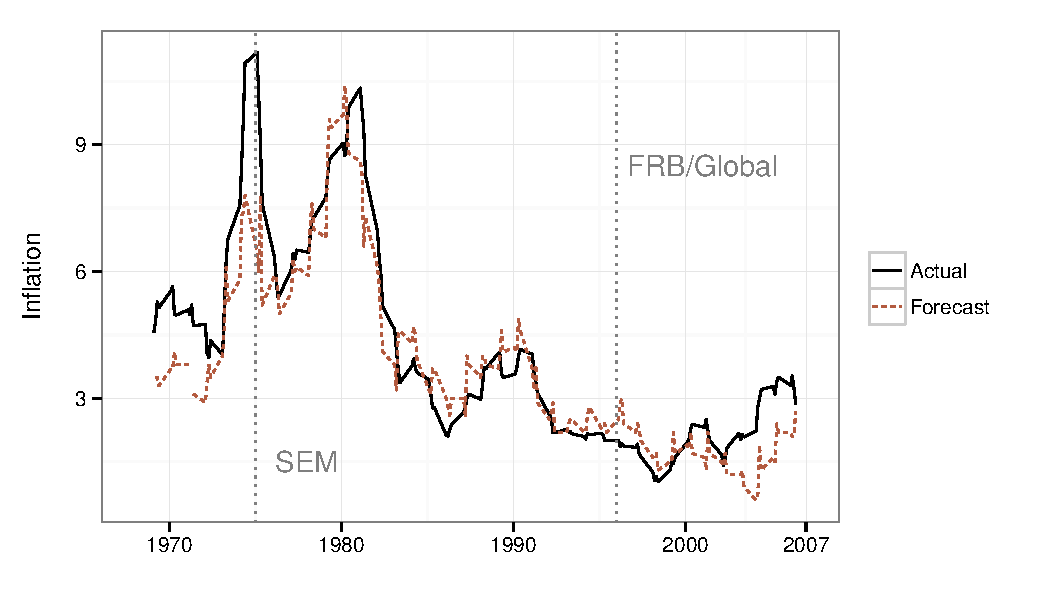
\includegraphics[width=0.8\linewidth]{figure/BaseInflation} 
\end{knitrout}

    
    \end{center}
    \begin{singlespace}
        {\scriptsize{Forecasts were made two quarters beforehand. \\
                     The grey dotted lines indicate the {\emph{approximate}} years that the Simultaneous Equation Models (SEM) and Federal Reserve Board Global (FRB/Global) forecasting models were fully implemented.  
                      }}
    \end{singlespace}
\end{figure}


\subsection{Are There Partisan Forecast Errors?}




Forecasts should be unbiased in that they have a mean error of zero \citep[5]{Bruck2006}. Using this criteria, forecast errors should be the same--ideally with a mean of 0--regardless of the incumbent president's party identification. This is not the case. From the second quarter of 1969 through 2006 the mean standardized forecast error was -0.03, i.e. forecasts were off by about -3 percent. However, the mean  forecast error across Republican presidencies was -11 percent and 13 percent across Democratic presidencies.\footnote{These means are from estimates made two quarters beforehand. Both means are statistically significantly different from 0, the full observation mean, and each other at the 99\% confidence level. For more details see \url{http://bit.ly/WHsRYh}.} On average, inflation was underestimated in Republican presidencies and overestimated in Democratic ones.

Figure \ref{errors_over_time} plots forecast errors across our sample. The first thing to note is that inflation was rarely underestimated during the three Democratic presidential terms in our sample. The underestimates that were made were relatively small. Also, the largest overestimates were made during Clinton's (Democratic) presidency. All of the major inflation underestimates were made during Republican presidencies, particularly during Nixon's, Ford's, and George W. Bush's presidencies. Inflation was often overestimated during the second part of Reagan's first term, his second term and George H.W. Bush's term. Over this period--often referred to as the Volcker Revolution \citep[see][]{Bartels1985}--inflation was suddenly much lower than before, (see Figure \ref{absolute}). It may have taken awhile for predictions to adjust to this new lower level of inflation, particularly because the Fed's own models of the economy assumed that money had no real effects on the economy during this period (see above).

This summary examination of inflation forecast errors suggests that there may be a partisan bias. What might explain this?

%%%%%%%%%%%%%%%%%%%%%%%%%%   Green Book Error Across Time
\begin{figure}[t]
    \caption{Errors in Inflation Forecasts Made 2 Qtr. Beforehand (1969 - 2006)}
    \label{errors_over_time}
    \begin{center}
    
\begin{knitrout}
\definecolor{shadecolor}{rgb}{0.969, 0.969, 0.969}\color{fgcolor}\includegraphics[width=0.8\linewidth]{figure/PartisanError} 
\end{knitrout}

    
    \end{center}
    \begin{singlespace}
        {\scriptsize{Note: An error of 0 indicates that inflation was perfectly predicted.}}
    \end{singlespace}
\end{figure}


%%%%%%%%%%%%%%%%%%%%%%%%%%%%% Section 2: Possible Explanations of Fed Inflation Forecast (In)accuracy %%%%%%%%%
\section{Possible Explanations of Fed Inflation Forecast (In)accuracy}

In this section we try to understand trends in Fed inflation forecast errors by discussing theories from the the political economy literature that provide possible explanations of why forecasts seem to have a partisan bias. 

\subsection{Econometric Models \& Accuracy}

Before digging into the partisan explanations of forecast errors, which would largely be the result of Federal Reserve staff judgement, it is worth hypothesizing that perhaps forecast (in)accuracy is the result of systematic errors in the Staff's predictive econometric models. Presumably, the move to rational expectations ought to improve forecast accuracy relative to the earlier period. The goal of incorporating forward looking actors into the models was to account for an important source of endogeneity in the earlier models that could lead to overestimates of important economic indicators under some circumstances and underestimates of those same indicators under others. None of these over or underestimates, however, ought to have been linked to the party of the president. We would, however, expect that the magnitude of forecast errors' changed after 1996.

%Random thought: what if the models assume that voters have partisan expectations and behave according to those partisan characteristics. Then when the partisans fail to do so or when voters react to these as they should (by not reacting) this results in over or under-shooting inflation by the Fed, particularly under the early model?

% That's a good thought. It is a bit of a tweak on our argument, but not a fundamental challenge. To give it weight we need to talk to Fed staff I think.

\subsection{Partisan Biases \& Accuracy}

There is an extensive literature looking for partisan effects in monetary policy, but no studies examining the impact of presidential partisanship on predictions of inflation. Studies have looked for evidence of partisan preferences manifesting themselves in the monetary policies chosen by the FOMC. There are two essential reasons that partisan effects would be found in policy: either a preference for one party over another by members of the FOMC or an expectation that the parties will engage in systematically different policies that will influence inflation leading the Fed supports more preferred policies and attempts to inhibit less preferred ones. 

The preference arguments assume that a conservative central banker will prefer the election of politicians who hold more similar inflationary preferences (i.e., those with a stronger preference for low inflation). In the US this would mean that the Federal Reserve would implement policies that supported the electoral prospects of Republican incumbents and harm the electoral prospects of Democratic incumbents \citep{Clark2012,Hakes1988,Sieg1997,Tootell1996}.

The rational partisan expectations literature assumes that central bankers do not have an innate preference for one party over another, but instead expect Democrats and Republicans to behave differently in office \citep{Alesina1991,Hibbs1994}. It is these behavioral expectations that would lead to different monetary policy outcomes under Democratic and Republican presidencies with the former engaging in more expansionary and inflationary policies than the latter. In order to stave off a rise in inflation under a Democrat the Fed would tighten monetary policy (raise interest rates or reduce the money supply); because Republicans are expected to prefer low inflation, they will pursue low inflation policies and so the FOMC can accommodate Republican presidents policies without fear of stoking inflation. This argument is again based on the assumed preferences of partisans, but does not require the FOMC to be politically biased as the former does. 

Arguments similar to those in the literature on partisan monetary cycles can also be applied to predicting differences in inflation forecasts. We present three theoretical arguments about how inflation expectations would differ by the President's party: the partisan preference theory, the monetary expectations theory, and the partisan heuristics theory (see Figure \ref{ExpectGraphs} for an illustration of the theories' contrasting inflation error predictions). Of
the three, we find the partisan heuristics theory to be both most consistent with the data.




% Define colors for figure
%% See: http://colorbrewer2.org/
\definecolor{DEM}{HTML}{2259B3}
\definecolor{REP}{HTML}{C42B00}

\begin{figure}
  \caption{Stylized Inflation Forecast Error Predictions}
  \label{ExpectGraphs}
  \begin{center}

    \vspace{0.25cm}

    \tikzstyle{bagMain} = [text width = 5cm]
    \tikzstyle{bagDem} = [text = DEM]
    \tikzstyle{bagRep} = [text = REP]

\begin{tikzpicture}

  %%%% Partisan Preferences
  \node (PP) at (-7, 5) [bagMain]{{\bf{Partisan Preferences}}};
  \node (E) at (-10.5, 3.25) [bagMain, rotate=90]{{\emph{Forecast Error}}};
  \node (T) at (-7.3, -0.5) [bagMain]{{\emph{Duration of Pres. Term}}};
  
  \draw (-10, 0) -- (-6, 0);
  \draw (-10, 0) -- (-10, 4);
  
  \draw[color=REP, opacity=0.5] (-9.5, 2) -- (-7.5, 2); 
  \draw[color=DEM, opacity=0.5] (-9.5, 2) -- (-7.5, 2); 

  \draw[color=REP, opacity=0.5] (-7.5, 2) -- (-6.5, 1); 
  \draw[color=DEM, opacity=0.5] (-7.5, 2) -- (-6.5, 3); 

  \node (R1) at (-6.5, 0.5) [bagRep]{Rep.};
  \node (D1) at (-6.5, 3.5) [bagDem]{Dem.};

  
  %%%% Monetary Expectations
  \node (PP) at (-2, 5) [bagMain]{{\bf{Monetary Expectations}}};
  
  \draw (-5, 0) -- (-1, 0);
  \draw (-5, 0) -- (-5, 4);
  
  \draw[color=REP, opacity=0.5] (-4.5, 2) -- (-2.5, 2); 
  \draw[color=DEM, opacity=0.5] (-4.5, 2) -- (-2.5, 2); 

  \draw[color=DEM, opacity=0.5] (-2.5, 2) -- (-1.5, 1); 
  \draw[color=REP, opacity=0.5] (-2.5, 2) -- (-1.5, 3); 

  \node (D2) at (-1.5, 0.5) [bagDem]{Dem.};
  \node (R2) at (-1.5, 3.5) [bagRep]{Rep.};
  
  
  %%%% Partisan Heuristics
  
  \node (PP) at (3, 5) [bagMain]{{\bf{Partisan Heuristics}}};
  
  \draw (0, 0) -- (4, 0);
  \draw (0, 0) -- (0, 4);
  
  \draw[color=DEM, opacity=0.5] (0.5, 3) -- (4, 3); 
  \draw[color=REP, opacity=0.5] (0.5, 1) -- (4, 1); 

  \node (D3) at (3.5, 3.5) [bagDem]{Dem.};
  \node (R3) at (3.5, 0.5) [bagRep]{Rep.};

  \end{tikzpicture}
  \end{center}
\end{figure}




The {\bf{partisan preference theory}} of inflation forecast errors is similar to the partisan preference model of monetary policy described above. This theory assumes that Fed staff have a preference for more inflation averse politicians to control the executive and so produce inflation forecasts that would justify the implementation of easy monetary policy under Republican administrations and tight money under Democratic administrations, particularly as presidential elections approach. The FOMC, choosing policy based on these forecasts would then implement monetary policies to optimize its utility function, which would not need to depend upon presidential partisanship. However, because Fed staffers prefer low inflation to high, they would not necessarily want to produce too loose/tight monetary policy over an entire four year term. Instead, they would want to encourage an economic boost/contraction near the end of a Republican/Democratic presidency. This implies that realized inflation would be higher than forecast during Republican presidencies and lower than forecast for Democratic presidencies. These effects would be particularly pronounced in the {\emph{quarters running-up to elections}} as Fed staff attempt to help their favored political party \citep{Beck1987,Grier1987}. Further, accounting for actual changes in monetary policy ought to increase the magnitude of partisan effects. This is because predictions of inflation during Republican presidencies, for example, will be lower than what the staff actually expects. If looser monetary policy is implemented in response to these low inflation forecasts than would have been chosen under the staff's true inflationary expectations, inflation will actually be higher than the staff's original forecast.

The {\bf{monetary expectations theory}} assumes that there is a partisan bias in the FOMC. It assumes that Federal Reserve economists believe members of the FOMC will engage in partisan monetary policy by lowering interest rates under conservative administrations and increasing them under liberal presidents. In this formulation, the Fed staff has no preference for one party over another, but knows that the FOMC does and so formulates estimates in order to counter the FOMC's policies \citep{Clark2012}. If Fed economists believe that the Open Market Committee will choose systematically higher than called for interest rates during Democratic presidencies and vice versa for Republicans, then, assuming they are interested in the implementation of optimal monetary policies, they would produce forecasts that are higher than expected during Republican administrations and the lower for Democrats; the {\emph{opposite of what is expected in the partisan preference theory}}. If the FOMC fails to note the compensation made by the Fed staff, then we would expect that after accounting for implemented policies inflation forecasts would be higher than or equal to realized inflation during Republican terms and lower than or equal to forecasts under Democratic administrations.\footnote{If the FOMC anticipated these compensatory biases in staff forecasts, then the FOMC would discount the Green Book estimates and continue to implement inflationary policies during Republican administrations and contradictory policies during Democratic ones. This would result in approximately correct inflation forecasts for both Republicans and Democrats since the forecasts would be biased in the direction of the FOMC's partisan bias rather than a ``true" no-policy-change forecast. However, we largely did not observe this.} If the Fed staff believes that the FOMC will engage in this behavior only when presidential elections are approaching, then we would expect no partisan differences in forecasts at the beginning of a presidency and but increasing divergence as the term wanes.%Christopher: I'm not entirely sure about this. I am certain that it would be higher than the ideal inflation rate, but lower than it would have been had they given their real estimates.
 
Finally, the {\bf{partisan heuristics theory}} proposes that Fed staffers incorporate a heuristic \citep[see][]{kahneman1973, tverskykahneman1974, kahneman2003} about the policy behaviors of presidents from different parties and the effects these different policies will have on the economy. Heuristics, generally, are intuitions that reduce the complexity associated with making predictions. Though they can be useful ``sometimes they lead to severe and systematic errors" \citep[][1124]{tverskykahneman1974}. In this theory, economists at the Fed have an intuition that Democrats and Republicans behave differently in government and so formulate inflationary expectations with this in mind. If this intuition does not accurately correspond to how presidents actually act, or how their policies affect inflation, forecasts would be systematically biased: overestimates for Democratic presidents, underestimates for Republicans. There is evidence that Democratic and Republican presidents do not, in fact, differ significantly in their overall levels of spending \citep{Bartels2008}, so any expectation that they would pursue policies that would differentially affect inflation would be innacurate. These biases should be constant {\emph{across presidential terms}}, in contrast to the partisan preference and monetary expectation theories.

This model does not require that forecasters be conscious of their heuristics, but simply for it to work its way subtly into forecasts, particularly in the subjective aspect of the ``consensus forecast" put forth in the Green Book. Further, because this bias would not need to be conscious, the systematic error could easily go unnoticed (as mistakes could occur for any number of economic reasons that they have been trained to consider). If the bias goes unnoticed, then it will not be corrected in future inflation predictions. This differs from the {\bf{rational partisan expectations theory}} described above in the monetary policy outcome literature in two ways. First, because these beliefs are not updated to account for the lack of partisan differences in spending they are not ``rational". Second, and relatedly, this theory is based on psychological instead of game theoretic reasoning, which allows for the persistence of suboptimal strategies in a way that would be less likely in a rational choice model of this same process given the assumption that the goals of the actors are the same in the two models. % I think we might want to discuss how this contrasts with rational partisan expectations. 


%%%%%%%%%%%%%%%%%% Section 3: Research Methods %%%%%%%%%%%%%%%%%%

\section{Research Methods}

In order to test for the three potential types of partisan bias described above we use non-matched and matched data sets with parametric models \citep[see][]{Ho2007} to assess whether or not there is a partisan biases in Green Book inflation forecasts. This section discusses the choice of methods and variables. In the following section we discuss our results.

\subsection{Matching \& Models}

We are interested in disentangling the effects of presidential party ID and elections from  many background factors, such as economic shocks and FOMC policy changes, that might create inflation forecast errors. As such, we consider presidential partisan identification and elections to be `treatments' that may impact inflation forecast errors. Democratic presidencies are considered to be treatments. Republican presidencies are `controls'.\footnote{Of course the selection of `treatment' and `control' groups in this context is arbitrary.} The quarter when a presidential election is held and the quarter before it are considered treatments and all other quarters are controls. Of course, given that we are working with observational data, other variables that have an impact on forecast errors may have {\emph{different distributions}} across the treatment and control groups \citep{Cochran1973, Diamond2012}. This makes it difficult to identify the relationships between presidential party ID, elections and errors from all of the confounding background variables.

To address this issue we follow the advice of \cite{Ho2007} to pre-process our data with matching to create data sets where the distributions of confounding variables are more even across treatment and control groups. We then run parametric analyses with the matched data sets. We used the {\tt{R}} package {\tt{MatchIt}} \citep{matchit2011} to create two matched data sets where the non-treatment covariates in the control groups closely matched those in the treatment groups. Doing this helps us isolate the effects of the `treatments' from that of the background covariates. 

Formally, each unit $i$ in the data set is `assigned' to either the treatment group ($t_{i} = 1$) or the control group ($t_{i} = 0$). $y_{i}(1)$ is the potential outcome--in our case the inflation forecast error--for unit $i$ of being in the treatment group, regardless of whether or not it was observed to be in this group. $y_{i}(0)$ is the potential outcome if $i$ was not in the treatment group, regardless of its observed assignment. It is impossible to observe both $y_{i}(1)$ and $y_{i}(0)$ at the same time. Instead we observe one version of $y_{i}=t_{i}y_{i}(1)-(1-t_{i})y_i(0)$. For each $i$ there is a fixed vector of exogenous confounders $X_{i}$. Ideally $t_{i}$ and $X_{i}$ are independent. However, this is not necessarily the case. The point of matching is to reduce or eliminate the relationship between $t_{i}$  and $X_{i}$ by selecting, dropping, and/or duplicating data. Ideally this process matches one treated unit with one controlled unit that has the same values of $X_{i}$, i.e. the distribution of covariates is the same in the treated and control groups \citep{matchit2011}. This is known as ``covariate balance" \cite[1]{Diamond2012}. Using matching to balance a data set ``break[s] the link between the treatment variables and the pre-treatment controls", effectively replicating the conditions of a randomized experiment with observational data \cite[][2--3]{matchit2011}. 

Balance is usually achieved in matching through propensity scores: the probabilities that units were assigned the treatment given their covariates. The propensity score model is generally unknown \citep{Drake1993}. To find the propensity score model we use Diamond and Sekhon's \citeyearpar{Diamond2012} genetic matching method (GenMatch).\footnote{The method is implemented with {\tt{MatchIt}} The original source code for the exact matching models can be found at {\url{http://bit.ly/OFdA4u}}.} GenMatch is a multivariate method that uses an evolutionary search algorithm to automate the search for the propensity score model that creates maximum balance. This minimizes the ``challenging" process of ``manually and iteratively checking the propensity score" to determine covariate balance \citep[][2]{Diamond2012}. 


\subsection{Parametric Models}

Once we created our matched data sets we used two types of parametric models to examine the effects of our treatment variables on the continuous inflation forecast error variable.\footnote{Parametric models are from the \texttt{R} package \texttt{Zelig} \citep{Zelig2012}.} The first was ordinary least squares linear regression (i.e. OLS).\footnote{In {\tt{Zelig}} this is the {\tt{ls}} model.} The other type was Bayesian normal linear regression\footnote{In {\tt{Zelig}} this is the {\tt{normal.bayes}} model.} which is particularly useful for our limited sample as it makes ``valid small sample inferences via draws from the exact posterior" \citep[][38]{Zelig2012}. Please see \cite{Goodrich2007} for details about Bayesian normal linear regression.  See also \cite{Imai2008} for a discussion of how to combine non-parametric matching and parametric analysis in one research process. Because we used non-parametric matching methods, not only do we better isolate the treatments' effects from those of the background variables, but we also reduce our estimated causal effects' dependence on the type of model we choose \cite[200--201]{Ho2007}.

The generic parametric model we used is given by
%
\begin{equation}
    E_{q} = \alpha + \beta T_{q} + \beta X_{q} + \epsilon,
\end{equation}
%
where $T_{q}$ is the treatment for quarter $q$ and $X$ is a vector of covariates. 

\subsection{Variables}

In Section \ref{ForecastAcc} we discussed our dependent variable--inflation forecast errors. To examine possible partisan biases we are interested in whether US presidents' partisan identity and/or the existence of an upcoming presidential election affect these errors. To do this we created {\bf{president party identification}} and {\bf{election period}} variables. The president party ID variable is 1 when the president is a Democrat and 0 when they are a Republican. Since forecast error data is released on a quarterly basis, we consider a president to be sitting from the first quarter after the election.\footnote{Elections are held almost at the midpoint--early November--of an election year's fourth quarter. Presidents are sworn into office near the beginning--20 January--of the following year's first quarter.} We consider quarters to be in the election period either if the presidential election is held in that quarter or in the following quarter.\footnote{If $q_{e}$ is a quarter with an election then we code quarters $q_{e}$ and $q_{e-1}$ election quarters.}

To further examine whether or not Federal Reserve staff were taking into consideration an electoral business cycle either due to a partisan preference or the nearness of an election, we include a variable of the {\bf{quarters until the presidential election}}. This simply counts down from the quarter after the previous election.\footnote{There are 15 quarters before a United States presidential election quarter.} The quarters that included presidential elections were coded as 0. 

The partisan preference and monetary expectations theories both posit that president's party ID and elections have an interactive relationship with forecast errors. To examine this possibility we include an interaction between the president party ID and election period variables in the analyses.

The United States president does not set the level of government expenditure--one of the main non-monetary policy causes of inflation--by themselves. Instead, the president is constrained by the two houses of Congress. To examine whether or not Federal Reserve staff are taking into consideration the partisan composition of Congress as well as the president's party identification, we include a variable of {\bf{Democratic legislators as a proportion of Republican legislators}} in the House of Representatives as well as a similar variable for the partisan composition of the Senate. Data on the number of legislators with Republican and Democratic party IDs was found at infoplease.\footnote{See {\url{http://www.infoplease.com/ipa/A0774721.html}}. Accessed May 2012.} 

There are at least three possible ways that Congressional party identification may affect forecast errors. The first is simply the possibility that Federal Reserve staff with rational partisan expectations pay attention to the partisan control of a chamber of Congress {\emph{independent of}} the president's party identification.  For example, Fed staff could predict more inflation tolerant policies if Democrats control the House of Representatives regardless of the partisan control of the Senate and presidency.

Though they make different predictions, the other two ways that the partisan composition of Congress may affect forecast errors is through an interaction with the president's party ID. The first interaction theory is that Federal Reserve staff with simple rational partisan expectations would presumably expect that a Democratic president would be able to get policies closer to their ideal point when there is a Congress with similar preferences. If a Democratic president had chambers of Congress controlled by Democrats, presumably Federal Reserve staff would expect even higher fiscal expenditures and therefore even higher inflation. Conversely, Republican presidents with a Republican-controlled Congress may be even better at cutting spending, leading to even lower inflation.

The second interaction possibility is based largely on Krause's \citeyearpar{Krause2000} work about the affect of partisan divisions on fiscal deficits in the United States. He finds partisan fragmentation can play a role in increasing Federal deficits. Higher political conflict, he argues, ``results in equilibrium fiscal outcomes that favor greater spending and/or a willingness to lower taxes since politicians will exhibit a greater proclivity in providing voters with program benefits and to delay its payment" \citep[][542]{Krause2000}. Because of this Federal Reserve staff may anticipate higher government borrowing when the presidency and houses of Congress are controlled by different parties. 

However, if prediction errors are largely the result of systematically biased economic forecasting models we would expect errors to change overtime as the models changed. In particular, we would expect a decrease in the magnitude of errors to occur around 1996 when the Federal Reserve Board's new US and Global Behavioral Equation Model was introduced. To examine this we include a {\bf{FRB/Global Model}} dummy variable. It equals one for all quarters from the first quarter of 1996 onward. It is zero otherwise.

Green Book forecasts are based on the assumption that monetary policy will not change between when the prediction is made and the time period it is predicting. Forecast errors may occur if monetary policy changes. If this is the case monetary policy changes would have a negative relationship with forecast errors. When the FOMC raises interest rates inflation may decline, causing the original forecast to have been too high and vice versa. To control for monetary policy changes we include a variable of {\bf{standardized changes to the discount rate}} from the quarter the Green Book prediction was made to the quarter it is predicting.\footnote{We averaged the discount rate over each quarter. Then we used the average discount rates $D$ in each quarter $q$ to create the variable $\Delta D_{q}$ using the simple formula: $\Delta D_{q} = \frac{D_{q} - D_{q-2}}{D_{q}}$. Note that the Federal Reserve changed how it used the discount rate and referred it at the beginning of 2003. To address this issue we primarily used data on the United States' discount rate recorded by the International Monetary Fund through this time period. Their data only goes back to the fourth quarter of 1982. So, before that we use the discount rate. Both of these variables are found in the FRED database at the St. Louis Federal Reserve (accessed July 2012). } The discount rate is one of the Federal Reserve's main tools for influencing the interest rate, especially the Fed funds rate.\footnote{A similar {\bf{relative changes in the Fed funds rate}} variable was included in some preliminary analyses. However, it did not change the results substantially and was estimated to have a similar effect on errors as the discount rate variable.}

To examine if Federal Reserve inflation forecast errors are affected by actual levels of government expenditure we include the percentage of {\bf{current government expenditure to GDP}} and {\bf{government debt to GDP}}. 

To examine how broader economic factors may be related to forecast errors we include variables of {\bf{GDP output gaps}} and {\bf{recessions}}. The former is simply potential GDP as a percentage of real GDP. The latter is a dummy variable for whether or not the United States was in a recession. All of these variables are from the FRED database\footnote{Accessed June 2012.} and are in nominal terms. 

Finally, we include a variable for the sitting {\bf{Federal Reserve Board Chair}}.\footnote{Chairs for the years in our analysis are William McChesney Martin, Jr., Arthur Burns, G. William Miller, Paul Volcker, Alan Greenspan, and Ben Bernanke.}

\section{Results}

In this section we present results from a number of parametric model specifications. We primarily diagnose the matching models with distributions of propensity scores--the probability of a quarter being in the ``treated" group given its covariates--as well as quantile-quantile plots \citep{Ho2007} to diagnose whether or not each covariate in the matched data sets is balanced. Please see figures \ref{ElectPropensityScores} and \ref{PresPropensityScores} for the propensity score distributions in our matched data sets. The quantile-quantile plots are not shown, but can easily be created from by running the original matching models in our main analysis source code file.\footnote{The file is available at: \url{http://bit.ly/OFdA4u}.}  We are unable to achieve covariate balance for the Congressional interaction terms\footnote{The presidential party ID and election period interaction does balance.} and the Federal Reserve Chair variable.\footnote{Chairs in our data set in the pre-Volcker/Greenspan era as well as current Chair Ben Bernanke were in office for very few quarters, making it difficult to match them.} It is unlikely that we could achieve covariate balance on these interactions given our relatively small sample size. Because of this, we only discuss Congressional interaction term and Chair variable estimates from the non-matched data sets.

Almost all other parametric model specifications\footnote{Tables \ref{OutputEL} and \ref{OutputPL} do show interaction estimates from matched data sets for comparison with the non-matched results in Table \ref{OutputNL}.}} are run with both the matched and unmatched data sets. In all of the Bayesian regressions we use the {\tt{Zelig}} default 1,000 MCMC burn-in iterations and 10,000 iterations after burn-in. We use the Heidelberger-Welch diagnostic to examine whether or not the Markov Chains converged to their stationary distributions.

We also remove quarters from the sample where forecasters would not have known who the president would be because the president had not yet been elected for that quarter. For models where the dependent variable is forecasts made two quarters beforehand this means removing the 2 quarters following each presidential election.\footnote{In this case 19 quarters were removed.} Results from these restricted data sets are fairly similar to those from the full data set.

We graphically present the key results in this section. Coefficient estimate tables for the models are given in the Appendix (see tables \ref{OutputNL}, \ref{OutputEL}, \ref{OutputPL}, \ref{OutputNB}, and \ref{OutputPB}). In general there is very little difference between the coefficients estimated using OLS and Bayesian linear regression models (see Figure \ref{CoefComparePlots}). Usually more variables were `statistically significant' at the standard 0.05 significance level in models using unmatched data compared to estimates from the matched data sets.




\begin{figure}[t]
    \caption{95\% Confidence Bands for Coefficients from a Variety of Matching and Parametric Model Specifications}
    \label{CoefComparePlots}
    \begin{center}

\begin{knitrout}
\definecolor{shadecolor}{rgb}{0.969, 0.969, 0.969}\color{fgcolor}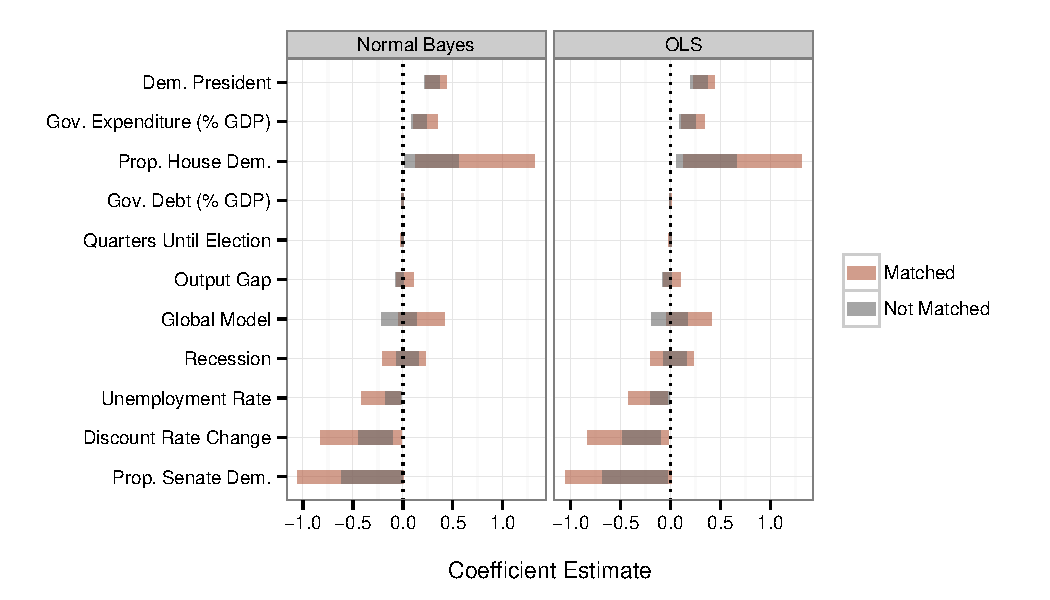
\includegraphics[width=0.95\linewidth]{figure/CoefComparePlots} 
\end{knitrout}

    \end{center}
    \begin{singlespace}
        {\scriptsize{Intercept values are not shown to maintain a reasonable scale for comparing covariate estimates. Please see the full estimates tables in the Appendix.}}
    \end{singlespace}
\end{figure}

\paragraph{Presidential Party Identification}

Our main finding is that presidential party identification had a strong positive association with Federal Reserve staff inflation forecast errors. Inflation forecast errors are estimated to be higher during Democratic presidencies than Republican ones even when we control for numerous other economic and political variables. This finding is what we would expect if Federal Reserve staff have a presidential partisan heuristic and is very robust across virtually all model specification using both matched and unmatched data.\footnote{The only models where the statistical significance of the variable drops below the 0.05 significance threshold is when it is interacted with both the House and Senate party variables using matched data. The matched data sets include relatively fewer observations, so these results may largely be because we are including more covariates in the models than the data has information to be able to draw meaningful conclusions for \citep{Brambor2006}.} Notably, the estimated effects hold even when we control for actual government expenditure. This suggests that Federal Reserve staff are not simply responding to different levels of government spending that Democratic and Republican presidents may tend to initiate, but either have a partisan preference or are using partisan heuristics.


\begin{figure}[t]
    \caption{Simulated Expected Inflation Forecast Error for Republican and Democratic Presidencies}
    \label{ExpectValueParty}
    \begin{center}

\begin{knitrout}
\definecolor{shadecolor}{rgb}{0.969, 0.969, 0.969}\color{fgcolor}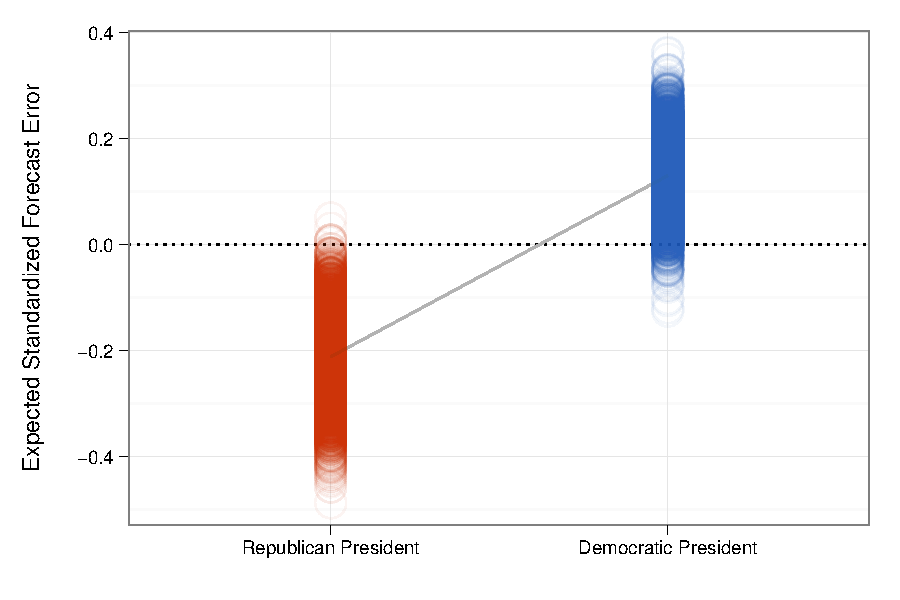
\includegraphics[width=0.75\linewidth]{figure/ExpectValueParty} 
\end{knitrout}



    \end{center}
    \begin{singlespace}
        {\scriptsize{Simulated from an OLS regression with data matched by presidential party identification. Variables included are generally the same as those in Model C7 from Table \ref{OutputPL}. The discount rate change variable is adjusted to reflect the change in the discount rate from the quarter when the forecast was made. Discount rate change was not included for the model predicting forecasts made in the present quarter since it is always 0. \\ The matching methods only include complete cases. Due to missing values early in the observation period we ran a different matching model for forecasts made three to five quarters beforehand. \\ Each model excludes every quarter when the forecasters would not have known who the president was. \\ The figure shows 950 simulations per presidential party ID type. They are the middle 95\% of 1000 simulations per presidential party ID type. \\ The solid line connects the two groups' means.}}
    \end{singlespace}
\end{figure}

To get a sense of approximately how big the presidential partisan ID bias might be we simulated expected standardized forecast errors for Democratic and Republican presidencies, holding the other covariates at their means.\footnote{We ran 1000 simulations on normal linear regression models matched by presidential party ID and including the same variables as those in Model C7 from Table \ref{OutputPL}.} Results from these simulations can be found in Figure \ref{ExpectValueParty}. For forecasts made two quarters in advance, we expect that on average the Fed overestimates inflation by 16 percent during Democratic presidencies. The average inflation error during Republican presidencies was approximately -27 percent. These estimates indicate that partisan biases are on average a fairly large contributor to the overall magnitude of inflation errors. This is clearly reflected in the large increase in the linear models' adusted $R^{2}$ when president partisan ID is included.\footnote{Compare the differences between the third and fourth models in tables \ref{NLTables}, \ref{ELTables}, and \ref{PLTables}.} 

There is some variation in the predicted error magnitude depending on how many quarters ago the forecast was made. Nonetheless it is notable that inflation is always predicted to be higher in Democratic presidencies than Republican presidencies. The distribution of the middle 95 percent of simulations for forecasts made three to five quarters beforehand occasionally overlap or come close to overlapping. This may largely be the result of the fact that we have far fewer observations for these estimates--due to missing data and dropping quarters with unknown presidents--which leads to much higher variance.

Clearly, at least between the 1970s and 2006, Fed staff were overly pessimistic about Democratic presidents' effect on inflation and even more overly optimistic about Republican presidents' effect. 

\paragraph{Presidential Elections}

Do Federal Reserve staff also take into consideration election timing as the partisan preference and monetary expectations theories predict? We do not find much if any evidence that inflation forecast errors were associated with elections either independent of presidential party ID or in interaction with it. This is true in parametric models using both unmatched and matched data where the election period variable is the treatment. Estimates of the relationship between the quarters until election variable and forecast errors\footnote{This variable is obviously omitted from the models with the election period variable because they are highly correlated.} also fails to provide any evidence that inflation errors are related to elections. 

We examined the monetary policy and partisan preference theories of forecast errors with an interaction between the president's party ID variable and the square of the time to election variable. We used the square to of the time to election variable to try to capture the non-linear predicted effect of the elections on errors in the monetary and partisan preference theories (see \ref{ExpectGraphs}. However, when we include the interactions the president's party ID variable is robust whereas the election variable and the interaction term are very statistically insignificant.\footnote{This is true when we use the non-squared version of the time to election variable.} This is reflected in the left-side graph in Figure \ref{InterPlot}.\footnote{This plot shows simulations from unmatched data. The results from models with matched data are virtually identical.} Inflation underestimates are predicted to become even worse as an election nears during Republican presidencies and slightly more overestimated close to elections for Democrats as the partisan preferences theory predicted. However it is important to note that this is not a statistically significant effect.

In this limited data set Fed Staff do not appear to be over estimating inflation when a Democratic president is running for reelection in an attempt to influence the FOMC to raise interest rates and lower the president's chances of winning as the partisan preference theory predicted. These findings have clear implications for how we understand the potential causes of Green Book partisan inflation forecast biases as well as FOMC interest rate decisions around elections. It seems that FOMC members, not their staff, are driving the increases in the Fed Funds Rate around elections when Democrats are in power that Clark and Arel-Bundock observed. 

Interestingly, staff also do not seem to compensate for FOMC partisan biases in an attempt to moderate FOMC-driven partisan electoral business cycles. Thus, we find no evidence in favor of the monetary expectations theory.

\paragraph{Partisan Control of Congress}

Might Federal Reserve staff be taking into consideration not only the president's party identification, but also the partisan composition of Congress?  Across all of our data sets and parametric model specifications we find no evidence that the partisan composition of congressional chambers independent of the president's party ID is related to inflation forecast errors. 

%%%%%%% President/Congress Interaction Plot %%%%%%%%
\begin{figure}[t]
    \caption{Simulated Expected Inflation Forecast Error with Interactions Between President Party ID and Quarters to Election$^{2}$, as well as President Party ID and Congressional Party Control (Non-matched data, Qtr. 2 forecasts)}
    \label{InterPlot}
    \begin{center}

\begin{knitrout}
\definecolor{shadecolor}{rgb}{0.969, 0.969, 0.969}\color{fgcolor}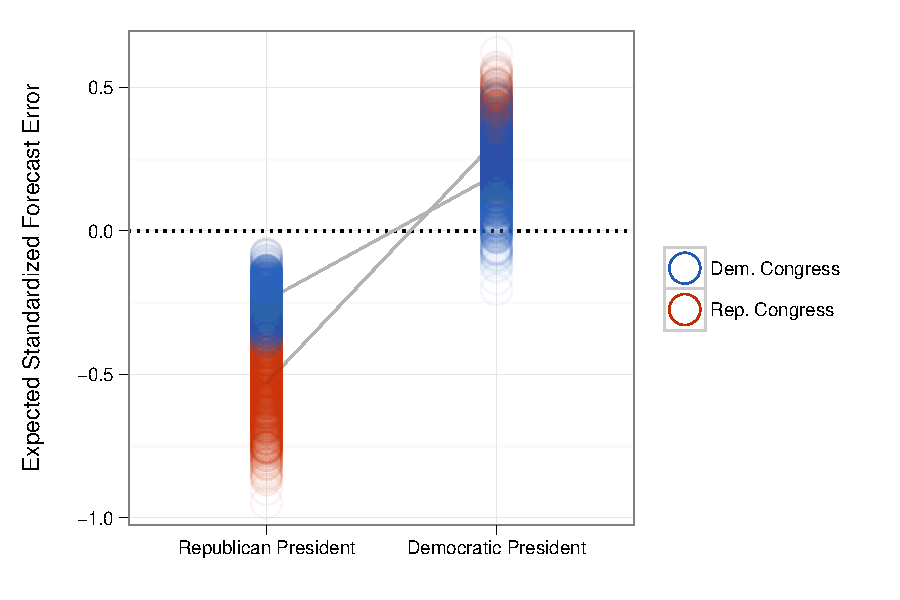
\includegraphics[width=0.95\linewidth]{figure/InterPlot} 
\end{knitrout}


    \end{center}
    \begin{singlespace}
        {\scriptsize{Simulated from OLS regressions with non-matched data. Expected errors in the left-side graph are from Model A8 in Table \ref{OutputNL} and the right-side estimates are from Model A11 from Table \ref{OutputPL}. The figure shows 950 simulations per fitted value. They are the middle 95\% of 1000 simulations per fitted value. \\ Both the House and Senate Democratic/Republican variables were set at 1.2 for Democratic congresses and 0.8 for Republican congresses. \\ The solid line connects the means of the congressional partisan control groups.}}
    \end{singlespace}
\end{figure}

We create parametric models using non-matched data with two-way and three-way interactions between presidential and congressional party identification to examine the two other ways we identified that presidential and congressional partisan ID might be related to forecast errors. All of the partisan interactions are generally statistically significant. To make substantive sense of these estimated interactions we again generate simulations to find expected inflation forecast errors at various levels of the presidential and congressional party identification. Figure \ref{InterPlot} shows simulation results from non-matched data with highly contrasting fitted variable values: one party control of the executive and both legislative bodies compared to a situation where one party controls the presidency and the other controls both houses of Congress.\footnote{Both the House and Senate Democratic/Republican variables are set at 1.2 for Democratic congresses and 0.8 for Republican congresses.} 

The first thing we should notice in Figure \ref{InterPlot} is how presidential partisan identification still seems to be driving the direction of the inflation forecast error: inflation is underestimated during Republican presidencies and overestimated during Democratic ones, regardless of what party controls Congress. The estimated substantive effect of congressional control on forecast errors is in the magnitude of the over or underestimates. In particular, Republican control of Congress seems to ecsasterbate the differences already noted between Democratic and Republican executives. Inflation is very underestimated for Republican presidencies with Republican congresses and more overestimated for Democratic presidents facing an opposition controlled legislature. There may be an expectation among Fed Staff that these governments will cut expenditure much more than they actually do. Forecast error is slightly higher on average with Democratic presidencies and Republican congresses compared to when both are controlled by Democrats. This finding fits with a story where Fed Staff believe spending will be higher with a divided government. 

Despite some evidence for an interaction between congressional and presidential party identification, it is not clear at this time how these results can be consistently explained across Democratic and Republican presidencies. We should also reiterate the fact that these interactions are estimated using non-matched data, because we are not able to achieve covariate balance for the interactions terms.

\paragraph{Government Expenditure}

It seems that Federal Reserve staff may also overestimate the effect of government expenditure on inflation. This is indicated by a consistently positive and significant coefficient for the government expenditure variable, even when controlling for president's party ID. Perhaps this is because Fed staff not only have a presidential partisan heuristic, but also a similar government expenditure heuristic where expenditure is believed to have a larger impact on inflation than it really does.

\paragraph{FRB Global Forecasting Model}

The introduction of the FRB/Global behavioral equation forecasting model does not seem to have begun a new era of reduced inflation forecasting error. Across all of our matching and parametric model specifications, forecasts made after the introduction of this approach are not significantly more accurate than those made before it. 

\paragraph{Changes to the Discount Rate}

As expected, relative changes to the discount rate are often found to be negatively associated with inflation forecast errors. Increasing the discount rate could result in lower inflation than expected and vice versa. Controlling for FOMC policy does not change the estimated relationship between presidential party ID and errors. It should be noted that the results are not robust across all of the models, especially when we use matched data. 




\paragraph{Orthogonal Dependent Variable Diagnostic: Unemployment Forecast Errors}

As a final diagnostic we ran our analyses with a dependant variable that is orthogonal to inflation forecast errors. This is a further way to determine if the results, especially for presidential party ID, are being driven by unobserved time period specific effects that are common to all Federal Reserve staff forecasts. The orthogonal variable we examined was {\bf{standardized unemployment rate forecast errors}}.\footnote{Unemployment forecast errors are not strongly correlated with inflation forecast errors.The Pearson correlation coefficitent for forecasts made two quarters beforehand is -0.15 with a p-value of 0.06. It is not clear why Federal Reserve staff would have systematically different unemployment forecast errors when there is a Republican president and a Democratic president.} The variable captures the errors Fed staff make when forecasting the unemployment rate in the same way that the inflation forecast variable measures inflation forecast errors. Unemployment rate forecasts are also reported in the Green Book. The actual unemployment rate was found using the Federal Reserve's FRED database.\footnote{We focused on 2 quarter forecasts.}

Most of the effects we found using inflation forecast errors disappeared or decreased dramatically in terms of statistical significance and magnitude when unemployment rate errors were the dependent variable.\footnote{The analyses can be fully recreated using source code available at: \url{http://bit.ly/S1nKyl}.} The lack of a relationship between presidential party ID and unemployment forecast errors is reflected in Figure \ref{Unemployment} in the Appendix. Unlike in Figure \ref{errors_over_time}, it is very difficult to find any partisan pattern to the errors. This provides more evidence that the presidential partisan ID effect is a real contributor to Federal Reserve staff's inflation forecasting errors.

\section*{Discussion: Is there a partisan bias?}

Do Fed forecasts have a partisan bias? According to the evidence from our research: yes they do. Federal Reserve staff seem to have systematically overestimated inflation during Democratic presidencies and underestimated it during Republican ones for at least a 35 year period between 1970 and the end of 2006. This finding was robust across numerous model specifications where a variety of economic, bureaucratic and other political factors were controlled for. 

Interestingly, in light of recent research on FOMC policy-making, we found no relationship between inflation forecast errors and elections either independent of presidential party identification or in interaction with it. This suggests that any relationship between monetary policy decisions and US presidential election timing is neither the result of partisan preferences that Fed staff members may have, nor beliefs that Fed staff may hold about the FOMC's presidential election preferences. 

Given the consistency of the bias across presidential terms, it appears that Fed staff members' partisan inflation forecast bias may be the result of a partisan heuristic. Like heuristics generally, the partisan bias may help Fed staffers simplify very complex phenomenon, while also leading to systematic prediction errors. These errors may not have been noticed by staffers because, so far, few if any people either inside or outside of the Fed have been looking for them. Thus, we do not fully explain the phenomenon uncovered by Clark and Arel-Bundock that motivated this research. We find that inflation forecasts are consistently underestimated when Republicans hold the White House and are consistently overestimated during Democratic administrations. We cannot explain why they find a positive linear relationship between time in office and the interest rate during Democratic presidencies (where interest rates start low and rise throughout the term) and the negative linear relation when Republicans are in office (where interest rates start high and fall as elections near). We therefore cannot yet rule out their theory that the FOMC is not politically indifferent.

What are the monetary policy and electoral implications of Federal Reserve staff partisan bias? Our research so far is not able to tell. It does motivate future research and point in a clear direction. It may be that higher inflation forecasts during Democratic presidencies spur the FOMC to raise interest rates and dampen the money supply generally. The opposite could happen during Republican presidencies. If this is the case, the economy would be inadvertently stimulated during Republican presidencies and depressed during Democratic ones, with clear electoral implications. The economic voting literature has repeatedly found that poor economic performance results in less electoral support for incumbent presidents \citep[e.g.][]{Alvarez1998, Bloom1975, LewisBeck1988, Powell1993}. Thus, if these partisan biases in inflation forecasts are leading to more restrictive monetary policy during Democratic presidencies and more expansive monetary policy during Republican presidencies, the economic voting mechanism may run afoul of important normative concerns about democratic accountability. Determining the extent to which these biases are shaping monetary policy is therefore an important next step in understanding the linkage between Fed inflation forecasts and larger questions of democracy. This is a very important issue that needs further investigation.

\clearpage
\section*{Appendix}

\subsection*{Replication}

This paper was written using {\tt{knitr}} \citep{knitr2012}. It can be entirely replicated from data, analysis source code, and markup files available on our GitHub page at: {\url{https://github.com/christophergandrud/GreenBook}}. 

%%%%%%% Table of non-matched data with OLS parametric model %%%%%%%%

\begin{table}[ht]
    \caption{OLS Estimation of Covariate Effects on 2 Qtr. Inflation Forecast Error (non-matched data set)}
    \label{OutputNL}
    \vspace{0.25cm}
    \begin{center}
    {\tiny

 
\begin{tabular}{ l D{.}{.}{1}D{.}{.}{1}D{.}{.}{1}D{.}{.}{1}D{.}{.}{1}D{.}{.}{1}D{.}{.}{1}D{.}{.}{1}D{.}{.}{1}D{.}{.}{1}D{.}{.}{1}D{.}{.}{1}D{.}{.}{1} } 
\hline 
  & \multicolumn{ 1 }{ c }{ A1 } & \multicolumn{ 1 }{ c }{ A2 } & \multicolumn{ 1 }{ c }{ A3 } & \multicolumn{ 1 }{ c }{ A4 } & \multicolumn{ 1 }{ c }{ A5 } & \multicolumn{ 1 }{ c }{ A6 } & \multicolumn{ 1 }{ c }{ A7 } & \multicolumn{ 1 }{ c }{ A8 } & \multicolumn{ 1 }{ c }{ A9 } & \multicolumn{ 1 }{ c }{ A10 } & \multicolumn{ 1 }{ c }{ A11 } & \multicolumn{ 1 }{ c }{ A12 } & \multicolumn{ 1 }{ c }{ A13 } \\ \hline
 %                    & A1              & A2              & A3              & A4              & A5              & A6              & A7              & A8              & A9              & A10             & A11             & A12             & A13            \\ 
Intercept            & 4.1 ^{**}       & 4.0 ^{**}       & 4.1 ^{**}       & 4.6 ^{***}      & 4.5 ^{***}      & 4.5 ^{***}      & 4.5 ^{***}      & 4.2 ^{***}      & 4.6 ^{***}      & 4.6 ^{***}      & 4.1 ^{***}      & 3.1 ^*          & -1.8 ^{***}    \\ 
                     & (1.3)           & (1.3)           & (1.3)           & (1.0)           & (1.1)           & (1.1)           & (1.1)           & (1.1)           & (1.1)           & (1.0)           & (1.0)           & (1.3)           & (0.4)          \\ 
Recession            & 0.0             & -0.0            & 0.0             & 0.1             & 0.1             & 0.1             & 0.1             & 0.1             & 0.0             & 0.1             & 0.1             & 0.1             &                \\ 
                     & (0.1)           & (0.1)           & (0.1)           & (0.1)           & (0.1)           & (0.1)           & (0.1)           & (0.1)           & (0.1)           & (0.1)           & (0.1)           & (0.1)           &                \\ 
Debt/GDP             & -0.0            & -0.0            & -0.0            & -0.0 ^*         & -0.0 ^*         & -0.0            & 0.0             & 0.0             & -0.0            & -0.0            & -0.0            & 0.0             &                \\ 
                     & (0.0)           & (0.0)           & (0.0)           & (0.0)           & (0.0)           & (0.0)           & (0.0)           & (0.0)           & (0.0)           & (0.0)           & (0.0)           & (0.0)           &                \\ 
Expenditure/GDP      & 0.1 ^{***}      & 0.1 ^{***}      & 0.1 ^{***}      & 0.2 ^{***}      & 0.2 ^{***}      & 0.2 ^{***}      & 0.1 ^{***}      & 0.1 ^{**}       & 0.2 ^{***}      & 0.1 ^{***}      & 0.2 ^{***}      & 0.1 ^{***}      &                \\ 
                     & (0.0)           & (0.0)           & (0.0)           & (0.0)           & (0.0)           & (0.0)           & (0.0)           & (0.0)           & (0.0)           & (0.0)           & (0.0)           & (0.0)           &                \\ 
Output Gap           & -0.1 ^{***}     & -0.1 ^{***}     & -0.1 ^{***}     & -0.1 ^{***}     & -0.1 ^{***}     & -0.1 ^{***}     & -0.1 ^{***}     & -0.1 ^{***}     & -0.1 ^{***}     & -0.1 ^{***}     & -0.1 ^{***}     & -0.1 ^{***}     &                \\ 
                     & (0.0)           & (0.0)           & (0.0)           & (0.0)           & (0.0)           & (0.0)           & (0.0)           & (0.0)           & (0.0)           & (0.0)           & (0.0)           & (0.0)           &                \\ 
Discount Rate Change & -0.1            & -0.1            & -0.1            & -0.3 ^{**}      & -0.3 ^{**}      & -0.3 ^{**}      & -0.3 ^{**}      & -0.3 ^{**}      & -0.3 ^{**}      & -0.2 ^{**}      & -0.2 ^*         & -0.2 ^*         &                \\ 
                     & (0.1)           & (0.1)           & (0.1)           & (0.1)           & (0.1)           & (0.1)           & (0.1)           & (0.1)           & (0.1)           & (0.1)           & (0.1)           & (0.1)           &                \\ 
Qtr. to Election     &                 & 0.0             &                 &                 & 0.0             & 0.0             & 0.0             &                 & 0.0             & 0.0 ^*          & 0.0 ^*          & 0.0 ^*          &                \\ 
                     &                 & (0.0)           &                 &                 & (0.0)           & (0.0)           & (0.0)           &                 & (0.0)           & (0.0)           & (0.0)           & (0.0)           &                \\ 
Election Period      &                 &                 & -0.0            &                 &                 &                 &                 &                 &                 &                 &                 &                 &                \\ 
                     &                 &                 & (0.1)           &                 &                 &                 &                 &                 &                 &                 &                 &                 &                \\ 
Pres. Party ID       &                 &                 &                 & 0.3 ^{***}      & 0.3 ^{***}      & 0.3 ^{***}      & 0.3 ^{***}      & 0.3 ^{***}      & 0.3 ^{***}      & 1.0 ^{***}      & 1.1 ^{***}      & 1.6 ^*          & 2.2 ^{**}      \\ 
                     &                 &                 &                 & (0.0)           & (0.0)           & (0.0)           & (0.0)           & (0.1)           & (0.0)           & (0.1)           & (0.2)           & (0.7)           & (0.8)          \\ 
Senate Dem/Rep       &                 &                 &                 &                 &                 & -0.2            & -0.3            & -0.3 ^\dagger  &                 & -0.1            & -0.0            & 0.5             & 0.8 ^*         \\ 
                     &                 &                 &                 &                 &                 & (0.1)           & (0.2)           & (0.2)           &                 & (0.1)           & (0.1)           & (0.3)           & (0.3)          \\ 
House Dem/Rep        &                 &                 &                 &                 &                 & 0.2             & 0.2             & 0.2             &                 & 0.4 ^{**}       & 0.3 ^*          & 1.1 ^{***}      & 1.6 ^{***}     \\ 
                     &                 &                 &                 &                 &                 & (0.1)           & (0.1)           & (0.1)           &                 & (0.1)           & (0.1)           & (0.3)           & (0.3)          \\ 
FRB/GlobalModel      &                 &                 &                 &                 &                 &                 & -0.1            & -0.1            &                 &                 &                 &                 &                \\ 
                     &                 &                 &                 &                 &                 &                 & (0.1)           & (0.1)           &                 &                 &                 &                 &                \\ 
Qrt. Election2       &                 &                 &                 &                 &                 &                 &                 & 0.0             &                 &                 &                 &                 &                \\ 
                     &                 &                 &                 &                 &                 &                 &                 & (0.0)           &                 &                 &                 &                 &                \\ 
Pres*Qrt. Election2  &                 &                 &                 &                 &                 &                 &                 & -0.0            &                 &                 &                 &                 &                \\ 
                     &                 &                 &                 &                 &                 &                 &                 & (0.0)           &                 &                 &                 &                 &                \\ 
Burns                &                 &                 &                 &                 &                 &                 &                 &                 & 0.2             &                 &                 &                 &                \\ 
                     &                 &                 &                 &                 &                 &                 &                 &                 & (0.2)           &                 &                 &                 &                \\ 
Greenspan            &                 &                 &                 &                 &                 &                 &                 &                 & 0.2             &                 &                 &                 &                \\ 
                     &                 &                 &                 &                 &                 &                 &                 &                 & (0.1)           &                 &                 &                 &                \\ 
Martin               &                 &                 &                 &                 &                 &                 &                 &                 & 0.2             &                 &                 &                 &                \\ 
                     &                 &                 &                 &                 &                 &                 &                 &                 & (0.2)           &                 &                 &                 &                \\ 
Miller               &                 &                 &                 &                 &                 &                 &                 &                 & 0.1             &                 &                 &                 &                \\ 
                     &                 &                 &                 &                 &                 &                 &                 &                 & (0.2)           &                 &                 &                 &                \\ 
Volcker              &                 &                 &                 &                 &                 &                 &                 &                 & 0.2             &                 &                 &                 &                \\ 
                     &                 &                 &                 &                 &                 &                 &                 &                 & (0.2)           &                 &                 &                 &                \\ 
Pres*House           &                 &                 &                 &                 &                 &                 &                 &                 &                 & -0.5 ^{***}     &                 & -1.5 ^\dagger  & -2.5 ^{**}     \\ 
                     &                 &                 &                 &                 &                 &                 &                 &                 &                 & (0.1)           &                 & (0.8)           & (0.9)          \\ 
Pres*Senate          &                 &                 &                 &                 &                 &                 &                 &                 &                 &                 & -0.7 ^{***}     & -0.2            & -0.2           \\ 
                     &                 &                 &                 &                 &                 &                 &                 &                 &                 &                 & (0.1)           & (0.8)           & (0.7)          \\ 
House*Senate         &                 &                 &                 &                 &                 &                 &                 &                 &                 &                 &                 & -0.5 ^*         & -0.9 ^{***}    \\ 
                     &                 &                 &                 &                 &                 &                 &                 &                 &                 &                 &                 & (0.2)           & (0.2)          \\ 
Pres*House*Senate    &                 &                 &                 &                 &                 &                 &                 &                 &                 &                 &                 & 0.5             & 1.0 ^\dagger  \\ 
                     &                 &                 &                 &                 &                 &                 &                 &                 &                 &                 &                 & (0.5)           & (0.5)           \\
 $N$                  & 131             & 131             & 131             & 131             & 131             & 131             & 131             & 131             & 131             & 131             & 131             & 131             & 131            \\ 
$R^2$                & 0.3             & 0.3             & 0.3             & 0.5             & 0.5             & 0.5             & 0.5             & 0.5             & 0.5             & 0.6             & 0.6             & 0.6             & 0.5            \\ 
adj. $R^2$           & 0.3             & 0.2             & 0.2             & 0.5             & 0.5             & 0.5             & 0.5             & 0.5             & 0.5             & 0.6             & 0.6             & 0.6             & 0.5            \\ 
Resid. sd            & 0.2             & 0.2             & 0.2             & 0.2             & 0.2             & 0.2             & 0.2             & 0.2             & 0.2             & 0.2             & 0.2             & 0.2             & 0.2             \\ \hline
 \multicolumn{14}{l}{\footnotesize{Standard errors in parentheses}}\\
\multicolumn{14}{l}{\footnotesize{$^\dagger$ significant at $p<.10$; $^* p<.05$; $^{**} p<.01$; $^{***} p<.001$}} 
\end{tabular} 



    }
    \end{center}
\end{table}

%%%%%%% Table of ElectionPeriod matched data with OLS parametric model %%%%%%%%

\begin{table}[ht]
    \caption{OLS Estimation of Covariate Effects on 2 Qtr. Inflation Forecast Error (Matched by Election Period Variable)}
    \label{OutputEL}
    \vspace{0.25cm}
    \begin{center}
    {\footnotesize

 
\begin{tabular}{ l D{.}{.}{1}D{.}{.}{1}D{.}{.}{1}D{.}{.}{1}D{.}{.}{1}D{.}{.}{1}D{.}{.}{1}D{.}{.}{1}D{.}{.}{1}D{.}{.}{1}D{.}{.}{1}D{.}{.}{1} } 
\hline 
  & \multicolumn{ 1 }{ c }{ B1 } & \multicolumn{ 1 }{ c }{ B2 } & \multicolumn{ 1 }{ c }{ B3 } & \multicolumn{ 1 }{ c }{ B4 } & \multicolumn{ 1 }{ c }{ B5 } & \multicolumn{ 1 }{ c }{ B6 } & \multicolumn{ 1 }{ c }{ B7 } & \multicolumn{ 1 }{ c }{ B8 } & \multicolumn{ 1 }{ c }{ B9 } & \multicolumn{ 1 }{ c }{ B10 } & \multicolumn{ 1 }{ c }{ B11 } & \multicolumn{ 1 }{ c }{ B12 } \\ \hline
 %                    & B1              & B2              & B3              & B4              & B5              & B6              & B7              & B8              & B9              & B10             & B11             & B12            \\ 
Intercept            & 3.8             & 3.9             & 3.7             & 2.6             & 2.7             & 4.5             & 1.8             & 1.8             & 3.1             & 2.4             & -1.7            & -3.2 ^{***}    \\ 
                     & (3.3)           & (3.3)           & (3.3)           & (2.9)           & (2.9)           & (3.2)           & (4.3)           & (4.4)           & (2.7)           & (3.0)           & (4.3)           & (0.8)          \\ 
Debt/GDP             & -0.0            & -0.0            & -0.0            & -0.0            & -0.0            & 0.0             & 0.0             & 0.0             & -0.0            & -0.0            & 0.0             &                \\ 
                     & (0.0)           & (0.0)           & (0.0)           & (0.0)           & (0.0)           & (0.0)           & (0.0)           & (0.0)           & (0.0)           & (0.0)           & (0.0)           &                \\ 
Expenditure/GDP      & 0.1 ^*          & 0.1 ^*          & 0.1 ^*          & 0.2 ^{***}      & 0.2 ^{***}      & 0.2 ^{**}       & 0.1             & 0.1             & 0.3 ^{***}      & 0.3 ^{***}      & 0.1             &                \\ 
                     & (0.1)           & (0.1)           & (0.1)           & (0.1)           & (0.1)           & (0.1)           & (0.1)           & (0.1)           & (0.1)           & (0.1)           & (0.1)           &                \\ 
Output Gap           & -0.1            & -0.1            & -0.1            & -0.1 ^\dagger  & -0.1 ^\dagger  & -0.1 ^*         & -0.0            & -0.0            & -0.1 ^*         & -0.1 ^*         & -0.0            &                \\ 
                     & (0.0)           & (0.0)           & (0.0)           & (0.0)           & (0.0)           & (0.0)           & (0.1)           & (0.1)           & (0.0)           & (0.0)           & (0.0)           &                \\ 
Discount Rate Change & -0.5            & -0.5            & -0.5            & -0.1            & -0.2            & 0.1             & 0.3             & 0.3             & 0.2             & 0.2             & 0.4             &                \\ 
                     & (0.3)           & (0.3)           & (0.3)           & (0.3)           & (0.3)           & (0.4)           & (0.4)           & (0.4)           & (0.3)           & (0.3)           & (0.3)           &                \\ 
Qtr. to Election     &                 & 0.0             &                 &                 & 0.0             & 0.0             & 0.0             &                 & 0.0             & 0.0             & 0.0 ^*          &                \\ 
                     &                 & (0.0)           &                 &                 & (0.0)           & (0.0)           & (0.0)           &                 & (0.0)           & (0.0)           & (0.0)           &                \\ 
Election Period      &                 &                 & 0.0             &                 &                 &                 &                 &                 &                 &                 &                 &                \\ 
                     &                 &                 & (0.1)           &                 &                 &                 &                 &                 &                 &                 &                 &                \\ 
Pres. Party ID       &                 &                 &                 & 0.3 ^{**}       & 0.3 ^{**}       & 0.4 ^{**}       & 0.4 ^{**}       & 0.5 ^{**}       & 1.4 ^{***}      & 1.6 ^{**}       & 1.0             & 0.6            \\ 
                     &                 &                 &                 & (0.1)           & (0.1)           & (0.1)           & (0.1)           & (0.1)           & (0.3)           & (0.5)           & (0.6)           & (0.4)          \\ 
Senate Dem/Rep       &                 &                 &                 &                 &                 & 0.0             & -0.1            & -0.2            & 0.4             & 0.5             & 2.4 ^*          & 2.1 ^*         \\ 
                     &                 &                 &                 &                 &                 & (0.3)           & (0.4)           & (0.4)           & (0.3)           & (0.4)           & (1.1)           & (0.8)          \\ 
House Dem/Rep        &                 &                 &                 &                 &                 & 0.4             & 0.2             & 0.2             & 0.1             & 0.0             & 2.3 ^{**}       & 2.3 ^{***}     \\ 
                     &                 &                 &                 &                 &                 & (0.4)           & (0.5)           & (0.5)           & (0.4)           & (0.4)           & (0.8)           & (0.5)          \\ 
FRB/GlobalModel      &                 &                 &                 &                 &                 &                 & -0.4            & -0.4            &                 &                 &                 &                \\ 
                     &                 &                 &                 &                 &                 &                 & (0.4)           & (0.4)           &                 &                 &                 &                \\ 
Qrt. Election2       &                 &                 &                 &                 &                 &                 &                 & 0.0             &                 &                 &                 &                \\ 
                     &                 &                 &                 &                 &                 &                 &                 & (0.0)           &                 &                 &                 &                \\ 
Pres*Qrt. Election2  &                 &                 &                 &                 &                 &                 &                 & -0.0            &                 &                 &                 &                \\ 
                     &                 &                 &                 &                 &                 &                 &                 & (0.0)           &                 &                 &                 &                \\ 
Pres*House           &                 &                 &                 &                 &                 &                 &                 &                 & -0.8 ^{**}      &                 & -2.6 ^{**}      & -2.7 ^{**}     \\ 
                     &                 &                 &                 &                 &                 &                 &                 &                 & (0.2)           &                 & (0.9)           & (0.7)          \\ 
Pres*Senate          &                 &                 &                 &                 &                 &                 &                 &                 &                 & -1.0 ^*         & 2.5             & 2.8 ^*         \\ 
                     &                 &                 &                 &                 &                 &                 &                 &                 &                 & (0.4)           & (1.5)           & (1.1)          \\ 
House*Senate         &                 &                 &                 &                 &                 &                 &                 &                 &                 &                 & -1.5 ^*         & -1.5 ^{**}     \\ 
                     &                 &                 &                 &                 &                 &                 &                 &                 &                 &                 & (0.6)           & (0.4)           \\
 $N$                  & 30              & 30              & 30              & 30              & 30              & 30              & 30              & 30              & 30              & 30              & 30              & 30             \\ 
$R^2$                & 0.3             & 0.3             & 0.3             & 0.5             & 0.5             & 0.5             & 0.6             & 0.6             & 0.7             & 0.6             & 0.8             & 0.7            \\ 
adj. $R^2$           & 0.2             & 0.1             & 0.1             & 0.4             & 0.4             & 0.4             & 0.4             & 0.3             & 0.6             & 0.5             & 0.7             & 0.6            \\ 
Resid. sd            & 0.2             & 0.3             & 0.3             & 0.2             & 0.2             & 0.2             & 0.2             & 0.2             & 0.2             & 0.2             & 0.2             & 0.2             \\ \hline
 \multicolumn{13}{l}{\footnotesize{Standard errors in parentheses}}\\
\multicolumn{13}{l}{\footnotesize{$^\dagger$ significant at $p<.10$; $^* p<.05$; $^{**} p<.01$; $^{***} p<.001$}}\\
\multicolumn{13}{l}{\footnotesize{The recession variable is ommitted because there was no variation in the matched data set.}}\\
\multicolumn{13}{l}{\footnotesize{The reason that there was no variation is because there was never a recession during an}}\\
\multicolumn{13}{l}{\footnotesize{election period in our data set.}} 
\end{tabular} 



    }
    \end{center}
\end{table}

%%%%%%% Table of pres_party matched data with OLS parametric model %%%%%%%%

\begin{table}[ht]
    \caption{OLS Estimation of Covariate Effects on 2 Qtr. Inflation Forecast Error (Matched by President's Party ID variable)}
    \label{OutputPL}
    \vspace{0.25cm}
    \begin{center}
    {\footnotesize

 
\begin{tabular}{ l D{.}{.}{1}D{.}{.}{1}D{.}{.}{1}D{.}{.}{1}D{.}{.}{1}D{.}{.}{1}D{.}{.}{1}D{.}{.}{1}D{.}{.}{1}D{.}{.}{1}D{.}{.}{1}D{.}{.}{1} } 
\hline 
  & \multicolumn{ 1 }{ c }{ C1 } & \multicolumn{ 1 }{ c }{ C2 } & \multicolumn{ 1 }{ c }{ C3 } & \multicolumn{ 1 }{ c }{ C4 } & \multicolumn{ 1 }{ c }{ C5 } & \multicolumn{ 1 }{ c }{ C6 } & \multicolumn{ 1 }{ c }{ C7 } & \multicolumn{ 1 }{ c }{ C8 } & \multicolumn{ 1 }{ c }{ C9 } & \multicolumn{ 1 }{ c }{ C10 } & \multicolumn{ 1 }{ c }{ C11 } & \multicolumn{ 1 }{ c }{ C12 } \\ \hline
 %                    & C1              & C2              & C3              & C4              & C5              & C6              & C7              & C8              & C9              & C10             & C11             & C12            \\ 
Intercept            & 6.3             & 6.4             & 6.5 ^\dagger   & 6.4 ^*          & 6.4 ^*          & 4.7             & 4.6             & 2.0             & 4.6             & 3.1             & 6.0             & -1.7 ^*        \\ 
                     & (3.8)           & (3.8)           & (3.8)           & (3.1)           & (3.2)           & (3.5)           & (3.6)           & (4.1)           & (2.8)           & (2.9)           & (3.9)           & (0.7)          \\ 
Recession            & 0.2             & 0.2             & 0.2             & 0.1             & 0.2             & 0.1             & 0.1             & 0.1             & 0.2             & 0.2             & 0.2             &                \\ 
                     & (0.2)           & (0.2)           & (0.2)           & (0.1)           & (0.2)           & (0.2)           & (0.2)           & (0.2)           & (0.1)           & (0.1)           & (0.1)           &                \\ 
Debt/GDP             & -0.0            & -0.0            & 0.0             & -0.0            & -0.0            & -0.0            & -0.0            & 0.0             & -0.0            & -0.0            & -0.0            &                \\ 
                     & (0.0)           & (0.0)           & (0.0)           & (0.0)           & (0.0)           & (0.0)           & (0.0)           & (0.0)           & (0.0)           & (0.0)           & (0.0)           &                \\ 
Expenditure/GDP      & 0.2 ^{**}       & 0.2 ^{**}       & 0.2 ^{**}       & 0.2 ^{***}      & 0.2 ^{***}      & 0.2 ^{**}       & 0.2 ^*          & 0.1 ^\dagger   & 0.2 ^{**}       & 0.2 ^{***}      & 0.2 ^*          &                \\ 
                     & (0.1)           & (0.1)           & (0.1)           & (0.1)           & (0.1)           & (0.1)           & (0.1)           & (0.1)           & (0.1)           & (0.1)           & (0.1)           &                \\ 
Output Gap           & -0.1 ^*         & -0.1 ^*         & -0.1 ^*         & -0.1 ^{**}      & -0.1 ^{**}      & -0.1 ^\dagger  & -0.1 ^\dagger  & -0.1            & -0.1 ^*         & -0.1 ^*         & -0.1 ^*         &                \\ 
                     & (0.0)           & (0.0)           & (0.0)           & (0.0)           & (0.0)           & (0.0)           & (0.0)           & (0.0)           & (0.0)           & (0.0)           & (0.0)           &                \\ 
Discount Rate Change & -0.3            & -0.3            & -0.2            & -0.5 ^\dagger  & -0.6 ^\dagger  & -0.5            & -0.5            & -0.5            & -0.4            & -0.3            & -0.5            &                \\ 
                     & (0.3)           & (0.3)           & (0.3)           & (0.3)           & (0.3)           & (0.3)           & (0.3)           & (0.3)           & (0.2)           & (0.3)           & (0.3)           &                \\ 
Qtr. to Election     &                 & 0.0             &                 &                 & 0.0             & 0.0             & 0.0             &                 & 0.0 ^*          & 0.0 ^\dagger   & 0.0 ^*          &                \\ 
                     &                 & (0.0)           &                 &                 & (0.0)           & (0.0)           & (0.0)           &                 & (0.0)           & (0.0)           & (0.0)           &                \\ 
Election Period      &                 &                 & 0.1             &                 &                 &                 &                 &                 &                 &                 &                 &                \\ 
                     &                 &                 & (0.1)           &                 &                 &                 &                 &                 &                 &                 &                 &                \\ 
Pres. Party ID       &                 &                 &                 & 0.3 ^{***}      & 0.3 ^{***}      & 0.3 ^{***}      & 0.3 ^{***}      & 0.4 ^{***}      & 1.3 ^{***}      & 1.5 ^{***}      & 1.1             & 2.1 ^*         \\ 
                     &                 &                 &                 & (0.1)           & (0.1)           & (0.1)           & (0.1)           & (0.1)           & (0.2)           & (0.2)           & (1.1)           & (1.0)          \\ 
Senate Dem/Rep       &                 &                 &                 &                 &                 & -0.4            & -0.3            & -0.6            & -0.1            & 0.0             & -0.3            & 0.5            \\ 
                     &                 &                 &                 &                 &                 & (0.3)           & (0.3)           & (0.4)           & (0.2)           & (0.2)           & (0.8)           & (0.7)          \\ 
House Dem/Rep        &                 &                 &                 &                 &                 & 0.1             & 0.1             & 0.5             & 0.6 ^*          & 0.4 ^\dagger   & 0.6             & 1.5 ^{**}      \\ 
                     &                 &                 &                 &                 &                 & (0.3)           & (0.3)           & (0.4)           & (0.2)           & (0.2)           & (0.7)           & (0.5)          \\ 
FRB/GlobalModel      &                 &                 &                 &                 &                 &                 & 0.0             & 0.0             &                 &                 &                 &                \\ 
                     &                 &                 &                 &                 &                 &                 & (0.1)           & (0.1)           &                 &                 &                 &                \\ 
Qrt. Election2       &                 &                 &                 &                 &                 &                 &                 & 0.0             &                 &                 &                 &                \\ 
                     &                 &                 &                 &                 &                 &                 &                 & (0.0)           &                 &                 &                 &                \\ 
Pres*Qrt. Election2  &                 &                 &                 &                 &                 &                 &                 & -0.0            &                 &                 &                 &                \\ 
                     &                 &                 &                 &                 &                 &                 &                 & (0.0)           &                 &                 &                 &                \\ 
Pres*House           &                 &                 &                 &                 &                 &                 &                 &                 & -0.8 ^{***}     &                 & -1.3            & -2.4 ^*        \\ 
                     &                 &                 &                 &                 &                 &                 &                 &                 & (0.1)           &                 & (1.2)           & (1.0)          \\ 
Pres*Senate          &                 &                 &                 &                 &                 &                 &                 &                 &                 & -1.0 ^{***}     & 0.8             & 0.2            \\ 
                     &                 &                 &                 &                 &                 &                 &                 &                 &                 & (0.2)           & (1.5)           & (0.9)          \\ 
House*Senate         &                 &                 &                 &                 &                 &                 &                 &                 &                 &                 & 0.0             & -0.6           \\ 
                     &                 &                 &                 &                 &                 &                 &                 &                 &                 &                 & (0.5)           & (0.4)          \\ 
Pres*House*Senate    &                 &                 &                 &                 &                 &                 &                 &                 &                 &                 & 0.0             & 0.8            \\ 
                     &                 &                 &                 &                 &                 &                 &                 &                 &                 &                 & (0.7)           & (0.6)           \\
 $N$                  & 60              & 60              & 60              & 60              & 60              & 60              & 60              & 60              & 60              & 60              & 60              & 60             \\ 
$R^2$                & 0.2             & 0.2             & 0.2             & 0.4             & 0.4             & 0.5             & 0.5             & 0.5             & 0.7             & 0.6             & 0.7             & 0.6            \\ 
adj. $R^2$           & 0.1             & 0.1             & 0.1             & 0.4             & 0.4             & 0.4             & 0.4             & 0.4             & 0.6             & 0.6             & 0.6             & 0.5            \\ 
Resid. sd            & 0.3             & 0.3             & 0.3             & 0.2             & 0.2             & 0.2             & 0.2             & 0.2             & 0.2             & 0.2             & 0.2             & 0.2             \\ \hline
 \multicolumn{13}{l}{\footnotesize{Standard errors in parentheses}}\\
\multicolumn{13}{l}{\footnotesize{$^\dagger$ significant at $p<.10$; $^* p<.05$; $^{**} p<.01$; $^{***} p<.001$}} 
\end{tabular} 



    }
    \end{center}
\end{table}

%%%%%%% Table of pres_party matched data with Bayesian normal linear parametric 

% latex table generated in R 2.15.2 by xtable 1.7-0 package
% Tue Nov  6 09:12:42 2012
\begin{table}[ht]
\begin{center}
\caption{Bayesian Normal Linear Regression Estimation of Covariate Effects on 2 Qtr. Inflation Forecast Error (non-matched data set)}
\label{OutputNB}
{\small
\begin{tabular}{lccccc}
  \hline
Variables & Mean & SD & 2.5\% & 50\% & 97.5\% \\ 
  \hline
Intercept & 4.49 & 0.99 & 2.56 & 4.49 & 6.46 \\ 
  Pres. Party ID & 0.30 & 0.04 & 0.22 & 0.30 & 0.38 \\ 
  Recession & 0.07 & 0.05 & -0.04 & 0.07 & 0.17 \\ 
  Qtr. to Election & -0.00 & 0.00 & -0.01 & -0.00 & 0.00 \\ 
  Senate Dem/Rep & -0.26 & 0.15 & -0.56 & -0.26 & 0.05 \\ 
  House Dem/Rep & 0.16 & 0.13 & -0.09 & 0.16 & 0.41 \\ 
  Debt/GDP & 0.00 & 0.00 & -0.01 & 0.00 & 0.01 \\ 
  Expenditure/GDP & 0.12 & 0.04 & 0.05 & 0.12 & 0.19 \\ 
  Output Gap & -0.07 & 0.01 & -0.10 & -0.07 & -0.04 \\ 
  Discount Rate Change & -0.27 & 0.09 & -0.44 & -0.27 & -0.10 \\ 
  Global Model & -0.10 & 0.08 & -0.27 & -0.10 & 0.06 \\ 
  sigma2 & 0.04 & 0.00 & 0.03 & 0.03 & 0.04 \\ 
   \hline
\end{tabular}
}
\end{center}
\end{table}





%%%%%%% Table of pres_party matched data with Normal Bayesian linear parametric model %%%%%%%%


% latex table generated in R 2.15.2 by xtable 1.7-0 package
% Tue Nov  6 09:12:42 2012
\begin{table}[ht]
\begin{center}
\caption{Bayesian Normal Linear Regression Estimation of Covariate Effects on 2 Qtr. Inflation Forecast Error (Matched by President's Party ID variable}
\label{OutputPB}
{\small
\begin{tabular}{lccccc}
  \hline
Variables & Mean & SD & 2.5\% & 50\% & 97.5\% \\ 
  \hline
Intercept & 4.60 & 3.74 & -2.70 & 4.59 & 11.90 \\ 
  Pres. Party ID & 0.34 & 0.08 & 0.19 & 0.34 & 0.49 \\ 
  Recession & 0.13 & 0.16 & -0.19 & 0.13 & 0.45 \\ 
  Qtr. to Election & 0.01 & 0.01 & -0.01 & 0.01 & 0.03 \\ 
  Senate Dem/Rep & -0.33 & 0.32 & -0.96 & -0.34 & 0.31 \\ 
  House Dem/Rep & 0.13 & 0.27 & -0.40 & 0.13 & 0.66 \\ 
  Debt/GDP & -0.00 & 0.01 & -0.02 & -0.00 & 0.01 \\ 
  Expenditure/GDP & 0.20 & 0.08 & 0.05 & 0.20 & 0.35 \\ 
  Output Gap & -0.08 & 0.05 & -0.18 & -0.08 & 0.01 \\ 
  Discount Rate Change & -0.46 & 0.34 & -1.12 & -0.46 & 0.20 \\ 
  Global Model & 0.02 & 0.15 & -0.27 & 0.02 & 0.31 \\ 
  sigma2 & 0.05 & 0.01 & 0.03 & 0.05 & 0.08 \\ 
   \hline
\end{tabular}
}
\end{center}
\end{table}





%%%%%%% Matching Diagnostic Plots %%%%%%
%%%%% Elections %%%%%%%
\begin{figure}[h]
  \caption{Matched on Election Period}
  \label{ElectPropensityScores}
\begin{knitrout}
\definecolor{shadecolor}{rgb}{0.969, 0.969, 0.969}\color{fgcolor}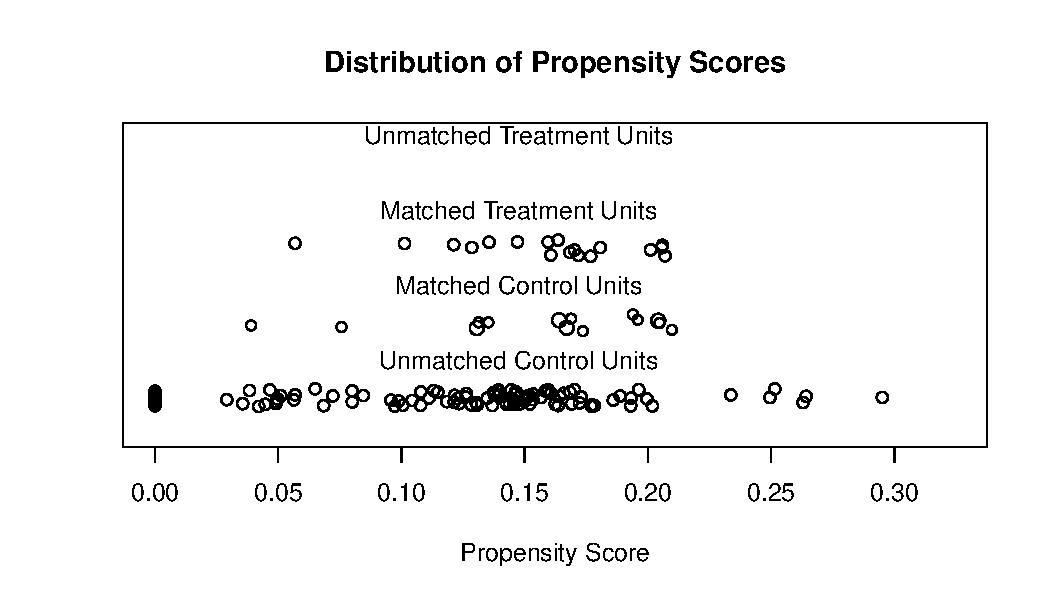
\includegraphics[width=\maxwidth]{figure/ElectPropensity} 
\end{knitrout}

    \begin{singlespace}
        {\scriptsize{Pre- and Post-matching propensity scores, where the ``Treated Units" are election quarters or the quarter before. ``Control Units" are from all other quarters. The more similar the distribution of matched treated and control unit propensity scores, the more successful the matching model was \cite[17]{Hollyer2012}.}}
    \end{singlespace}
\end{figure}

%%%%% Presidential Party ID %%%%%%
\begin{figure}[h]
  \caption{Matched on Presidential Party Identification}
  \label{PresPropensityScores}
\begin{knitrout}
\definecolor{shadecolor}{rgb}{0.969, 0.969, 0.969}\color{fgcolor}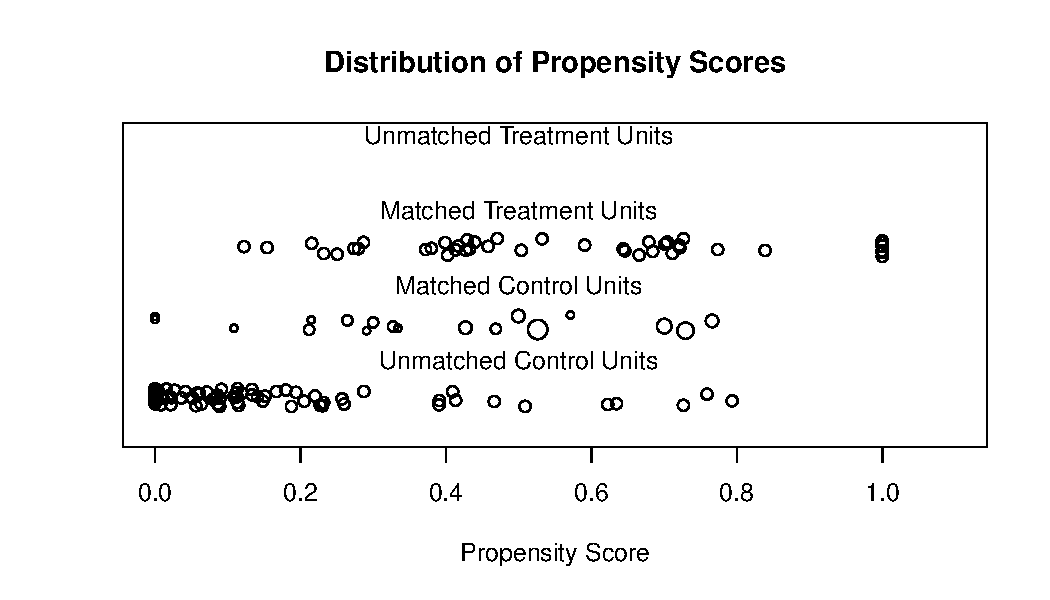
\includegraphics[width=\maxwidth]{figure/PresPropensity} 
\end{knitrout}

  \begin{singlespace}
      {\scriptsize{Pre- and Post-matching propensity scores, where the ``Treated Units" are quarters when the president was a Democrat. ``Control Units" are quarters when with a Republican president. The more similar the distributions of matched treated and control unit propensity scores, the more successful the matching model was \cite[17]{Hollyer2012}.}}
  \end{singlespace}
\end{figure}

%%%%%%%%%%%%%%%%%%%%%%%%%%   Green Book Unemployment Forecast Error Across Time
\begin{figure}[t]
    \caption{Diagnostics of Unemployment Rate Forecast Error as Orthogonal to Inflation Rate Forecast Errors for years 1969 - 2006}
    \label{Unemployment}
    \begin{center}
    
\begin{knitrout}
\definecolor{shadecolor}{rgb}{0.969, 0.969, 0.969}\color{fgcolor}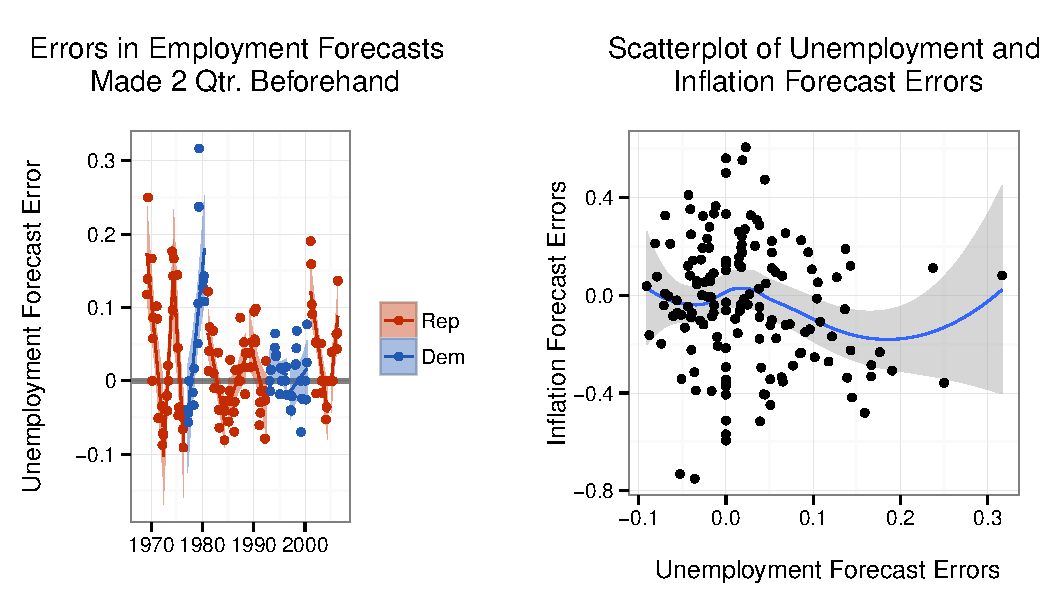
\includegraphics[width=0.95\linewidth]{figure/GraphPartisanErrorUnemploy} 
\end{knitrout}


    \end{center}
    \begin{singlespace}
        {\scriptsize{Note: Errors of 0 indicates that inflation/the unemployment rate was perfectly predicted.}}
    \end{singlespace}
\end{figure}


%%%%%%% References %%%%%%%%%%%%

\clearpage

\bibliographystyle{apsr}
\bibliography{GreenBook.bib}

\end{document}
